\documentclass{article}
\usepackage[utf8]{inputenc}
\usepackage[italian]{babel}
\usepackage{amsmath}
\usepackage{amssymb}
\usepackage{siunitx}
\usepackage{tabularray}
\usepackage{graphicx}
\usepackage{float}
\usepackage{xfrac}
\usepackage{caption}    % for \caption*{}
\usepackage[labelformat=simple, justification=centering]{subfig}
\renewcommand{\thesubfigure}{}
\newcommand*{\diam}{\varnothing}
\newcommand*{\best}[1]{{#1}_\text{best}}
\newcommand*{\bestp}[1]{{\left(#1\right)}_\text{best}}
\newcommand*{\pbest}[1]{\left({#1}_\text{best}\right)}
\newcommand*{\pbestp}[1]{\left({\left(#1\right)}_\text{best}\right)}
\newcommand*{\errrel}[1]{\frac{\delta #1}{{#1}_\text{best}}}
%% <custom footnotes/>
%\newcounter{savefootnote}
%\newcounter{symfootnote}
%\newcommand{\symfootnote}[1]{%
%   \setcounter{savefootnote}{\value{footnote}}%
%   \setcounter{footnote}{\value{symfootnote}}%
%   \ifnum\value{footnote}>8\setcounter{footnote}{0}\fi%
%   \let\oldthefootnote=\thefootnote%
%   \renewcommand{\thefootnote}{\fnsymbol{footnote}}%
%   \footnote{#1}%
%   \let\thefootnote=\oldthefootnote%
%   \setcounter{symfootnote}{\value{footnote}}%
%   \setcounter{footnote}{\value{savefootnote}}%
%}
%% </custom footnotes>
\title{
    Laboratorio di Fisica 1\\
    R8: Misura di $\left|\vec{g}\right|$ mediante rotolamento puro
}
\author{Gruppo 17: Bergamaschi Riccardo, Graiani Elia, Moglia Simone}
\date{19/03/2024 – 9/04/2024}
\makeindex
\begin{document}

\maketitle

\begin{abstract}
    Il gruppo di lavoro ha misurato indirettamente il modulo del campo gravitazionale locale ($g$)
    studiando il moto di rotolamento di un corpo rigido.
\end{abstract}

\setcounter{section}{-1}  % Count sections starting from 0
\section{Materiali e strumenti di misura utilizzati}
\begin{center}
    \begin{tblr}{
        width=\textwidth,
        colspec={ X[2,m,j]X[m,c]X[m,c]X[m,c] },
        vlines,
    }
        \hline
        \textbf{Strumento di misura} & \textbf{Soglia} & \textbf{Portata} & \textbf{Sensibilità} \\
        \hline
        {Sistema a contatti elettrici con contatore di impulsi} & \qty{1}{\micro s} & \qty{99999999}{\micro s} & \qty{1}{\micro s} \\
        \hline[dashed]
        Metro a nastro & \qty{0.1}{cm} & \qty{300.0}{cm} & \qty{0.1}{cm} \\
        \hline[dashed]
        Calibro ventesimale & \qty{0.05}{mm} & \qty{150.00}{mm} & \qty{0.05}{mm} \\
        \hline[dashed]
        Bilancia di precisione & \qty{0.01}{g} & \qty{4200.00}{g} & \qty{0.01}{g} \\
        \hline[dashed]
        Cellulare come goniometro & \qty{0.1}{\degree} & \qty{45.0}{\degree} & \qty{0.1}{\degree} \\
        \hline
    \end{tblr}
    \begin{tblr}{
        width=\textwidth,
        colspec={ X[m,j]X[3,m,j] },
        vlines,
    }
        \hline
        \textbf{Altro} & \textbf{Descrizione/Note} \\
        \hline
        Piano inclinato & {
            Costituito da guide che permettono al
            campione di cadere da un contatto elettrico
            all'altro con un moto di rotolamento puro.
        } \\
        \hline[dashed]
        Campione & {
            Corpo rigido con simmetria assiale,
            assimilabile a una combinazione di
            cilindri e tronchi di cono coassiali.
        } \\
        \hline[dashed]
        Cuscinetto & {
            Posto a coprire il secondo contatto
            elettrico, attutisce l'impatto del campione
            contro di esso.
        } \\
        \hline[dashed]
        Brugola e Lucidi & {
            Utili per cambiare, rispettivamente,
            la distanza tra i contatti e l'angolo
            di inclinazione delle guide.
        } \\
        \hline
    \end{tblr}
\end{center}

\section{Esperienza e procedimento di misura}
\begin{enumerate}
    \item
        Misuriamo la massa del campione con la bilancia di precisione
        e, con il calibro ventesimale, tutti i diametri e le altezze
        necessarie al calcolo del suo momento d'inerzia.
    \item
        Fissiamo la distanza $L$ tra i due contatti elettrici
        e l'angolo $\theta$ di inclinazione delle guide
        rispetto a un piano normale a $\vec{g}$.
        Allora, acceso e impostato adeguatamente il contatore
        di impulsi, misuriamo 50 volte il tempo di caduta del
        campione $t_{L,\theta}$.
    \item
        Ripetiamo il punto precedente per svariate combinazioni
        di $L$ e $\theta$.

\end{enumerate}

\section{Analisi dei dati raccolti e conclusioni}
\subsection{Calcolo del momento d'inerzia del campione}

Essendo il momento d'inerzia additivo, abbiamo calcolato
$I_\text{CM}$ sommando i singoli momenti d'inerzia rispetto al comune
asse di simmetria dei cilindri e dei tronchi di cono che compongono il
campione, dove la massa di ciascuno di essi è stata facilmente
calcolata assumendo la densità del campione uniforme.
Di seguito riportiamo tali misure:

\begin{table}[H]
    \centering

    \begin{tblr}{
        vlines = {},
        hline{1,2,17} = {},
        hline{3,5-7,9,10,12-14,16} = {dashed},
        cell{1,2,5,6,9,12,13,16}{1-5} = {c,m},
        cell{3,7,10,14}{1-3,5} = {r=2}{c,m},
    }
        $\#$&\emph{Forma}&$h\;(\unit{mm})$&$d_{1,2}\;(\unit{mm})$&$I\;(10^{-6}\;\unit{kg\,m^2})$\\
        1  & Cilindro          & $30.45\pm0.05$ & $49.90\pm0.05$ & $154.6 \pm1.8 $ \\
        2  & {Tronco\\di cono} & $ 5.95\pm0.10$ & $49.90\pm0.05$ & $ 13.7 \pm0.5 $ \\
           &                   &                & $29.40\pm0.05$ &                 \\
        3  & Cilindro          & $ 9.20\pm0.10$ & $25.85\pm0.05$ & $  3.36\pm0.08$ \\
        4  & Cilindro          & $10.80\pm0.05$ & $18.65\pm0.05$ & $  1.07\pm0.02$ \\
        5  & {Tronco\\di cono} & $ 4.25\pm0.05$ & $34.55\pm0.05$ & $ 11.8 \pm0.4 $ \\
           &                   &                & $49.90\pm0.05$ &                 \\
        6  & Cilindro          & $52.95\pm0.05$ & $49.90\pm0.05$ & $269   \pm3   $ \\
        7  & {Tronco\\di cono} & $ 4.25\pm0.05$ & $49.90\pm0.05$ & $ 12.6 \pm0.4 $ \\
           &                   &                & $36.35\pm0.05$ &                 \\
        8  & Cilindro          & $10.80\pm0.05$ & $18.75\pm0.05$ & $  1.09\pm0.02$ \\
        9  & Cilindro          & $ 9.25\pm0.10$ & $25.90\pm0.05$ & $  3.41\pm0.08$ \\
        10 & {Tronco\\di cono} & $ 5.95\pm0.10$ & $29.10\pm0.05$ & $ 13.5 \pm0.5 $ \\
           &                   &                & $49.90\pm0.05$ &                 \\
        11 & Cilindro          & $30.40\pm0.05$ & $49.90\pm0.05$ & $154.4 \pm1.8 $ \\
    \end{tblr}
\end{table}

\begin{itemize}
    \item Massa totale: $M=(2214.57\pm0.01)\;\unit{g}$
    \item Volume totale: $V=(2.654\pm0.017)\cdot10^{-4}\;\unit{m^3}$
    \item Densità media: $\rho=(8.34\pm0.05)\cdot10^{-3}\;\unit{kg \per m^3}$
    \item Momento d'inerzia totale: $I_\text{CM}=(6.38\pm0.09)\cdot10^{-4}\;\unit{kg\,m^2}$
\end{itemize}

\subsection{Distribuzione dei tempi di caduta}

Riportiamo di seguito i grafici della distribuzione dei tempi di caduta $t_{L,\theta}$,
accompagnati alle relative misure di $L$ e $\theta$.

\begin{figure}[H]
    \centering
    \subfloat[][
        $L=(55.6\pm0.1)\;\unit{cm}$

        $\theta=(3.8\pm0.1)\unit{\degree}$
    ]{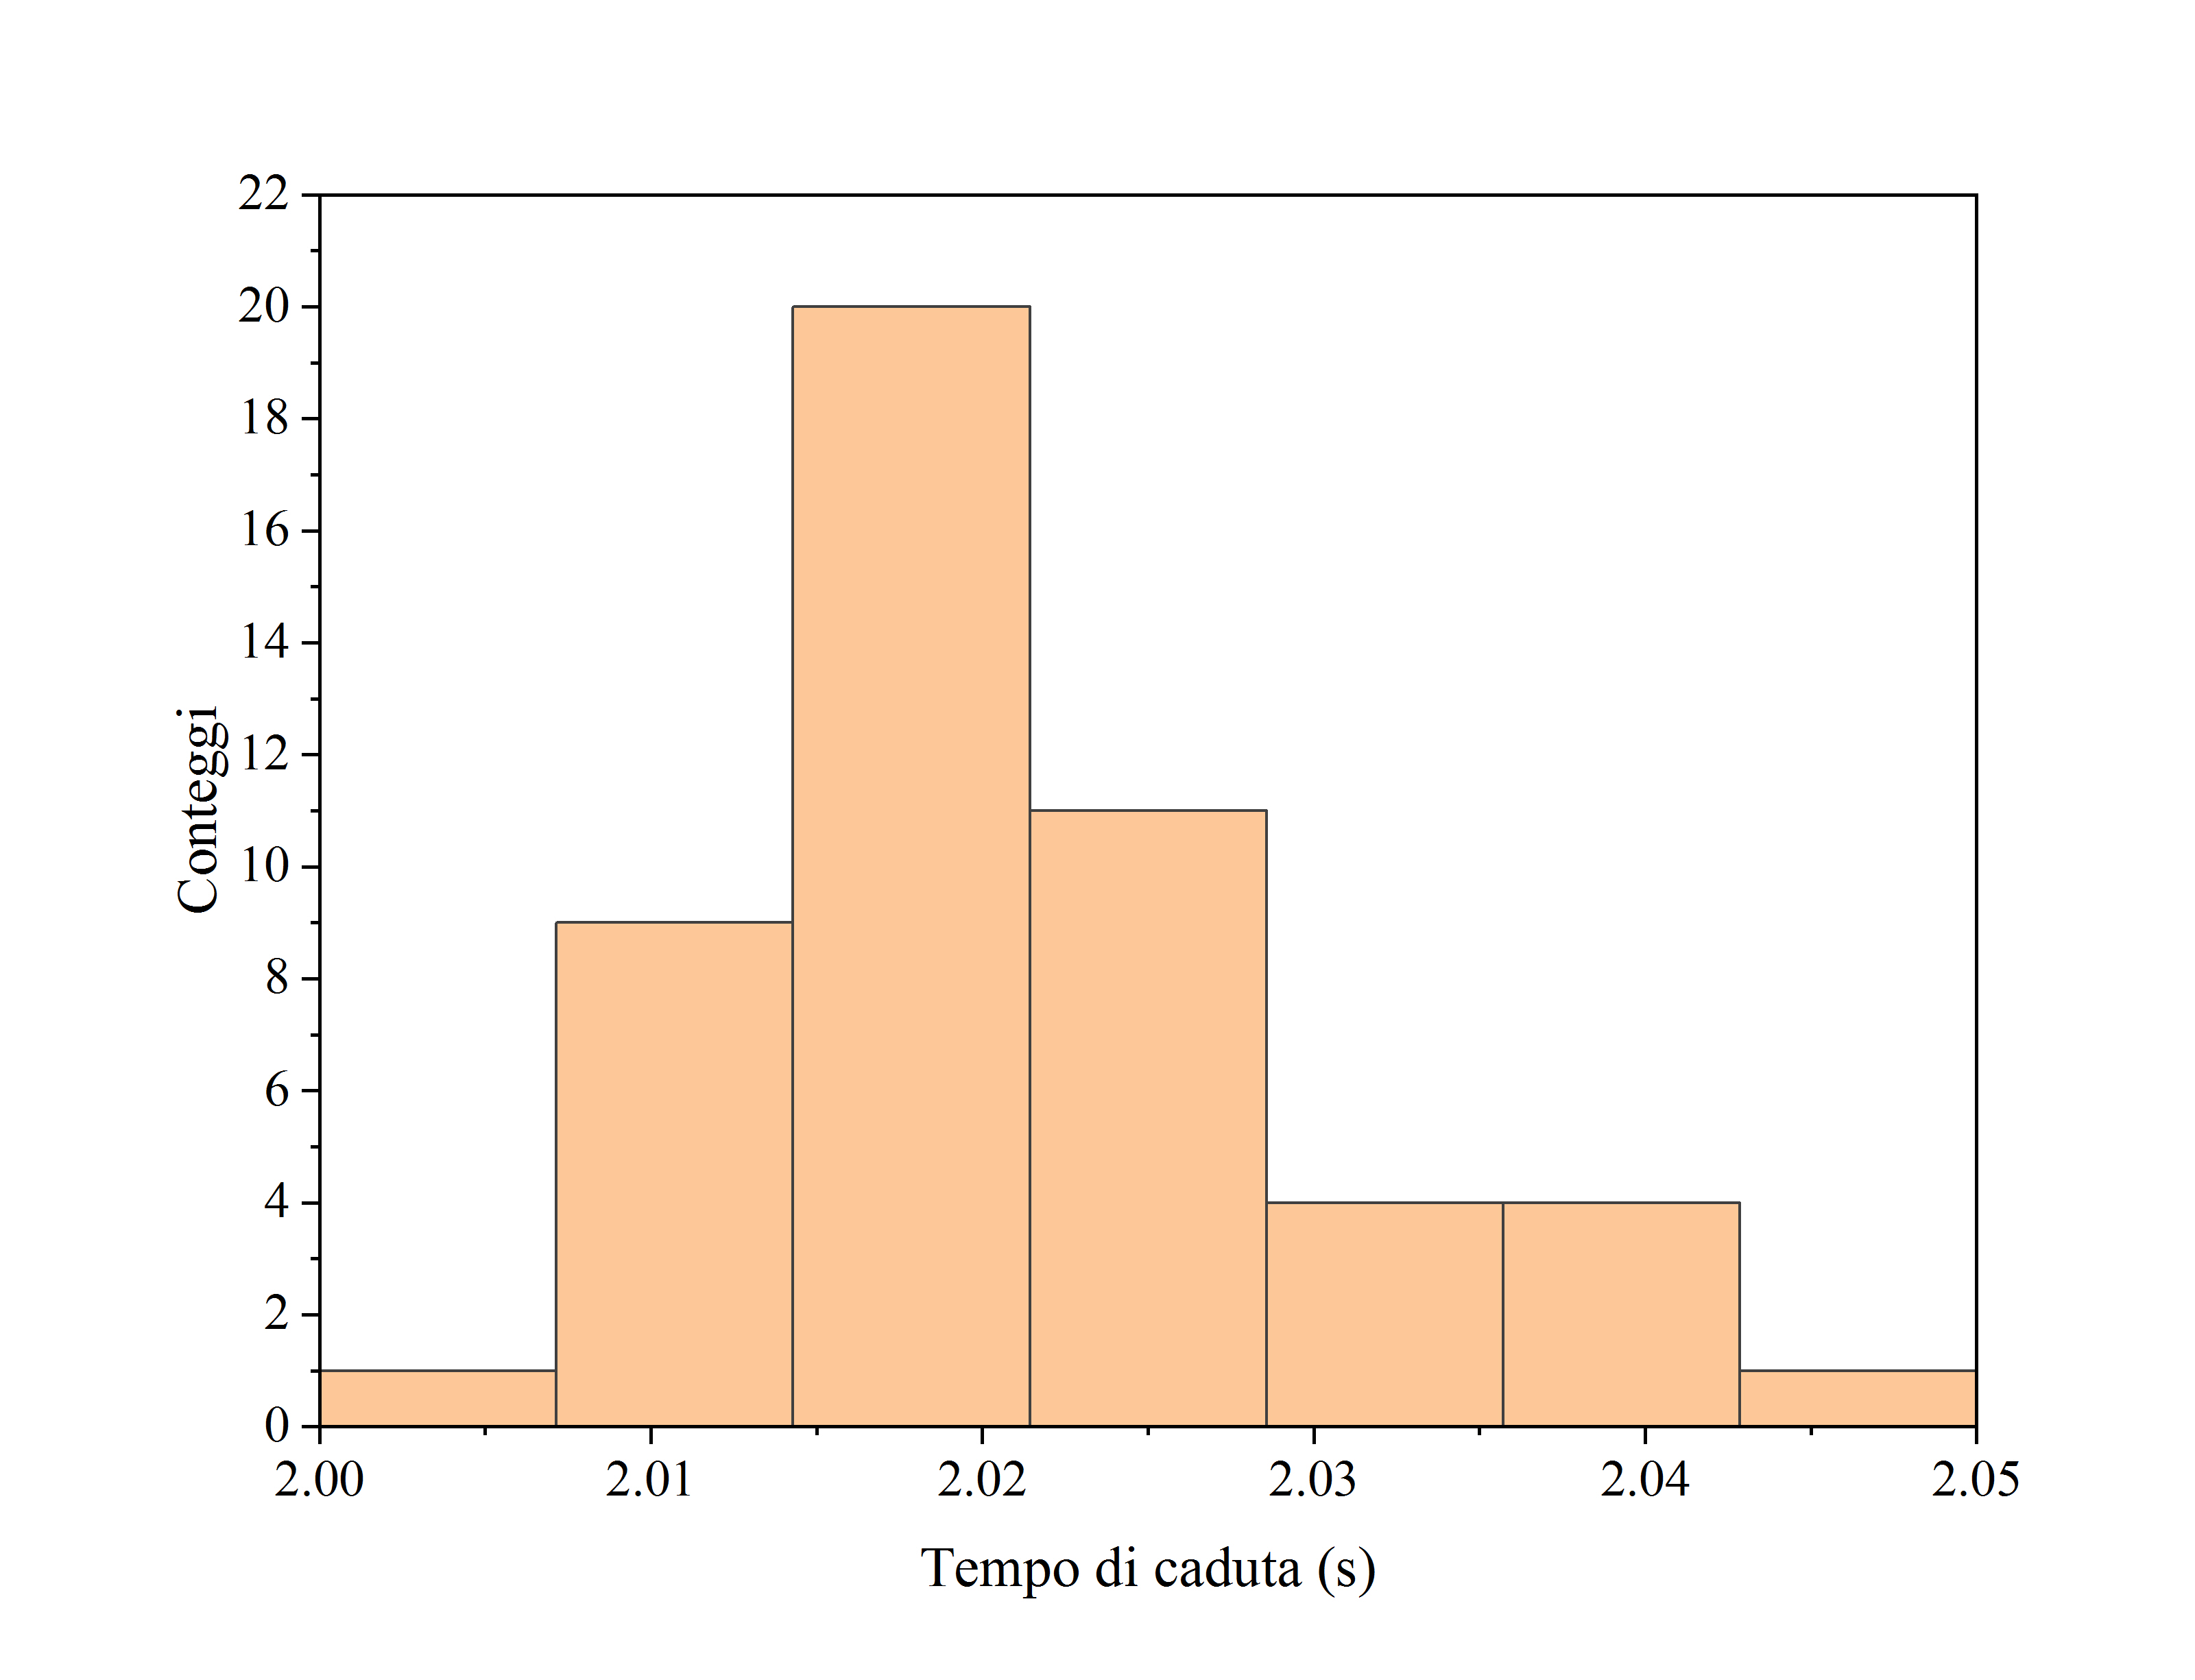
\includegraphics[trim={2.1cm 0.7cm 2.1cm 1cm},clip,width=0.47\textwidth]{img/G0.jpg}}\hfil
    \subfloat[][
        $L=(70.5\pm0.1)\;\unit{cm}$

        $\theta=(3.8\pm0.1)\unit{\degree}$
    ]{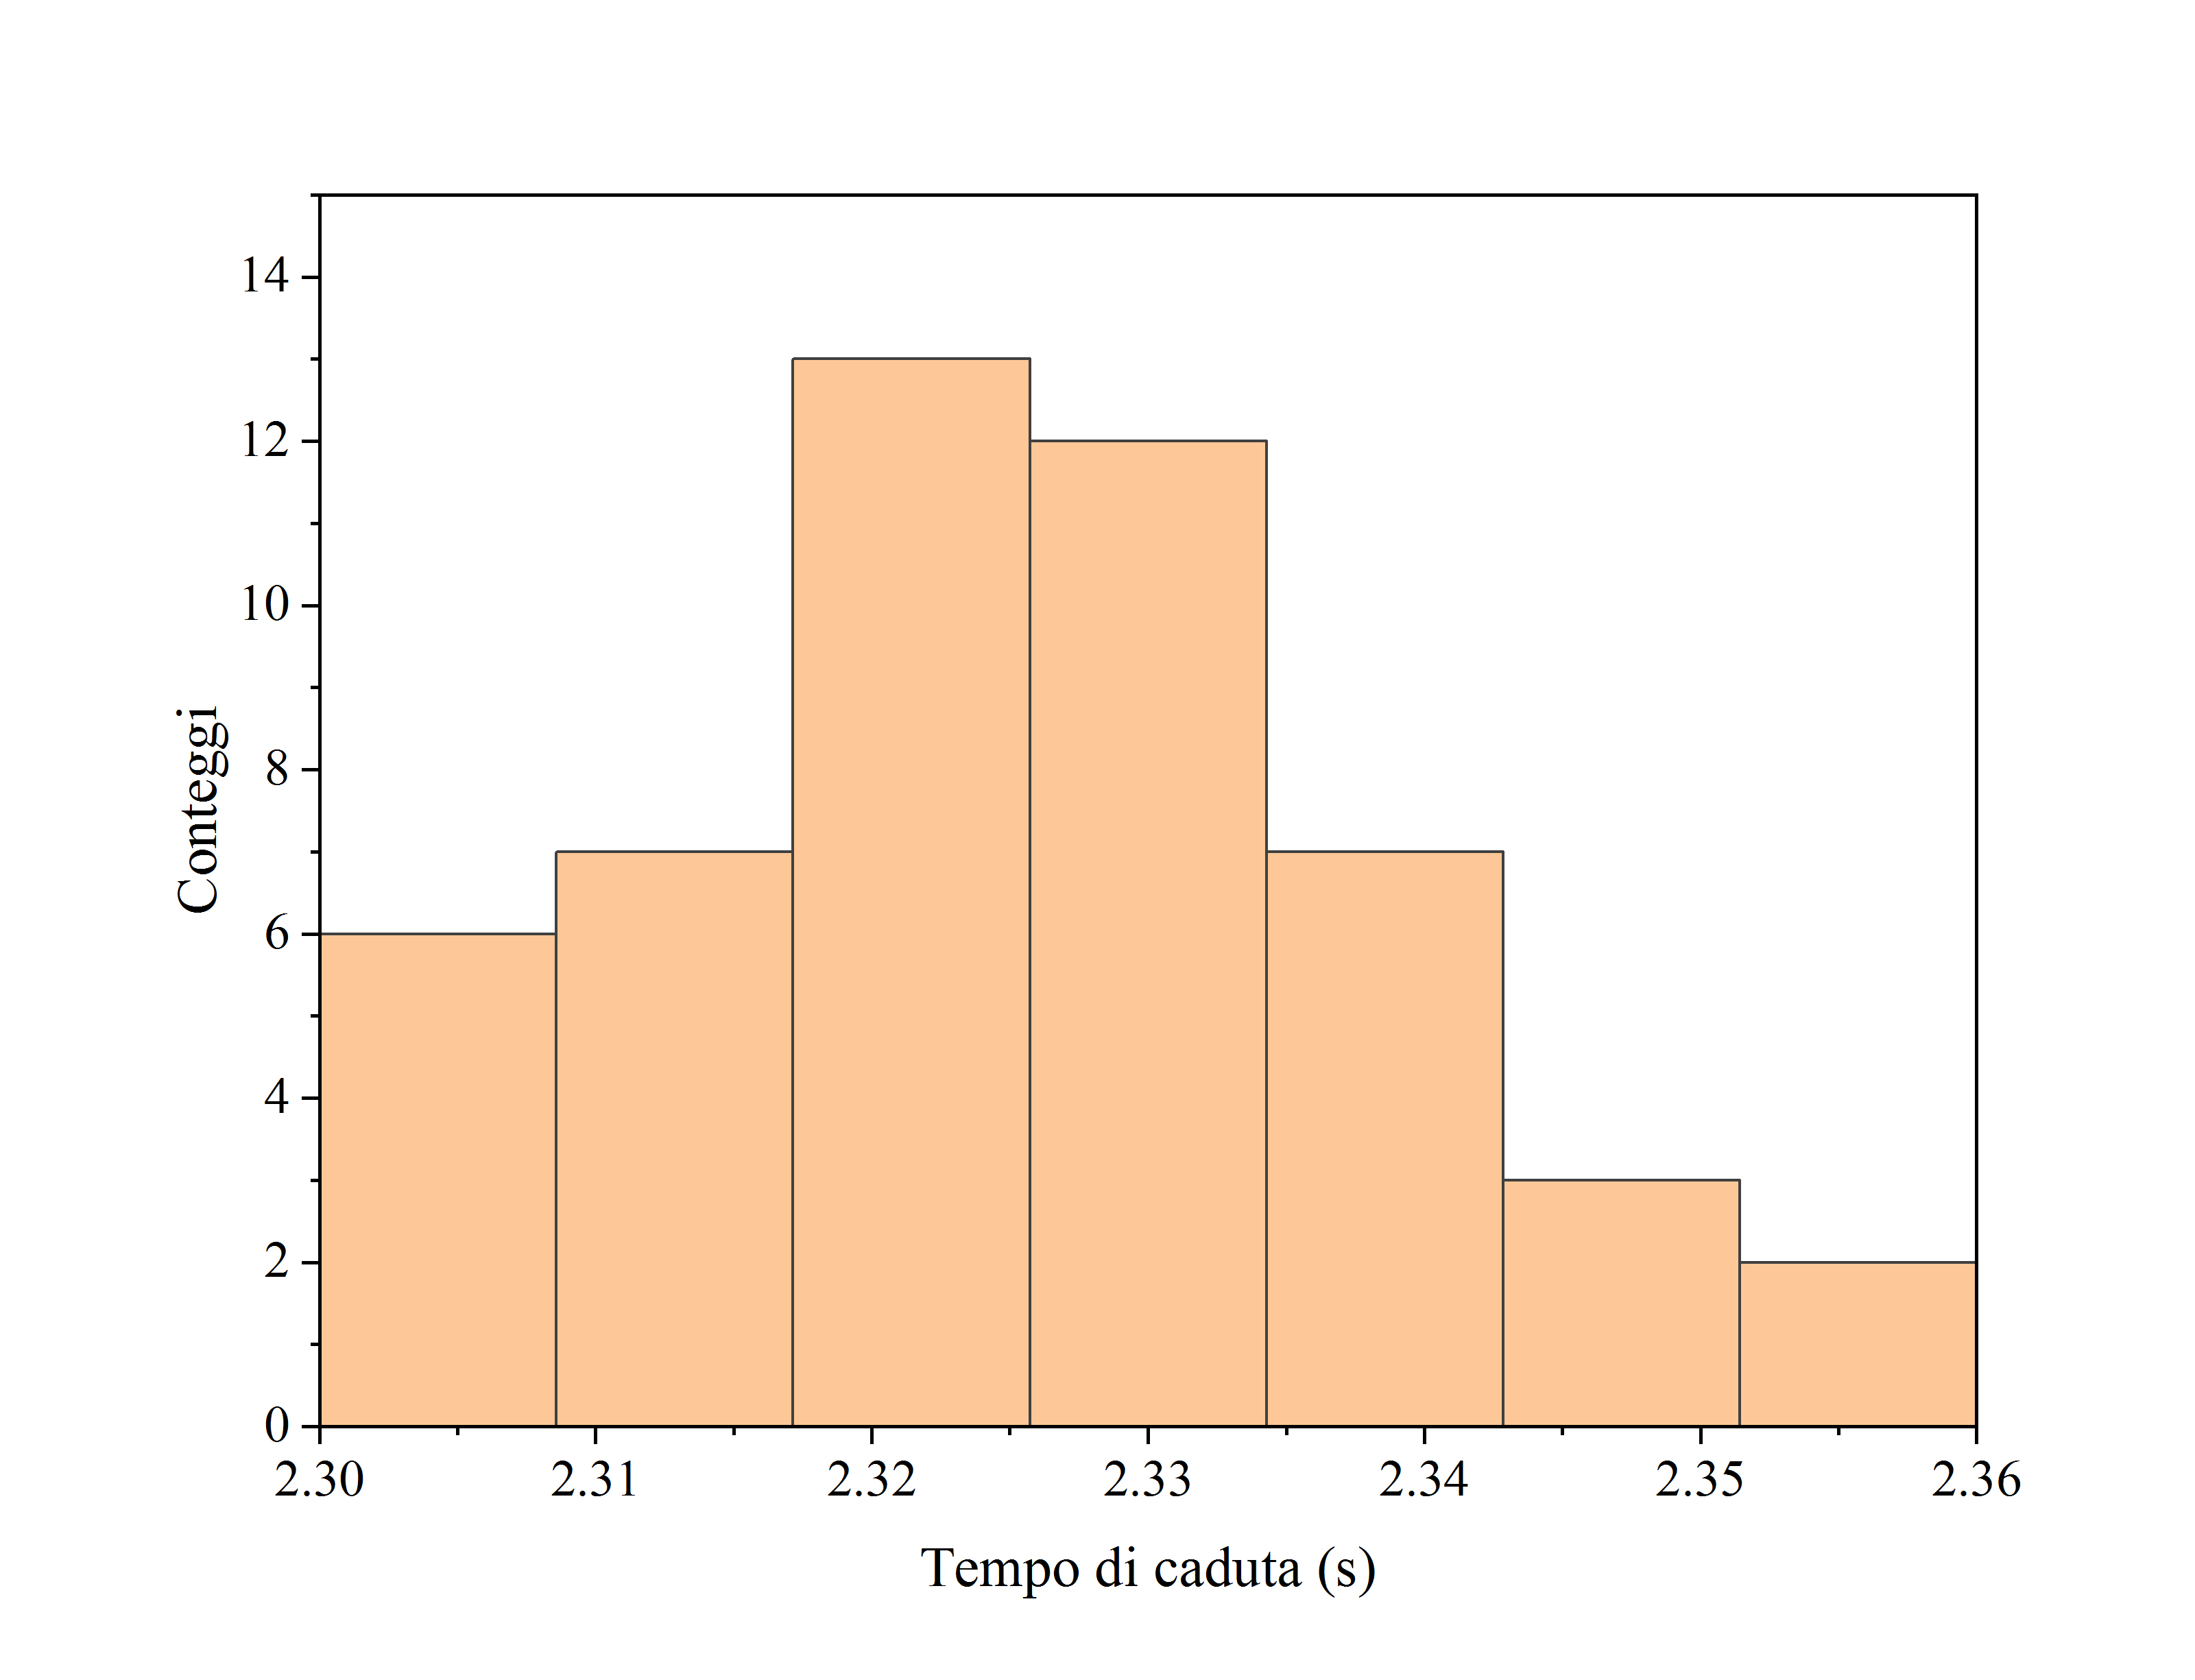
\includegraphics[trim={2.1cm 0.7cm 2.1cm 1cm},clip,width=0.47\textwidth]{img/G1.jpg}}\hfil
    \subfloat[][
        $L=(85.4\pm0.1)\;\unit{cm}$

        $\theta=(3.8\pm0.1)\unit{\degree}$
    ]{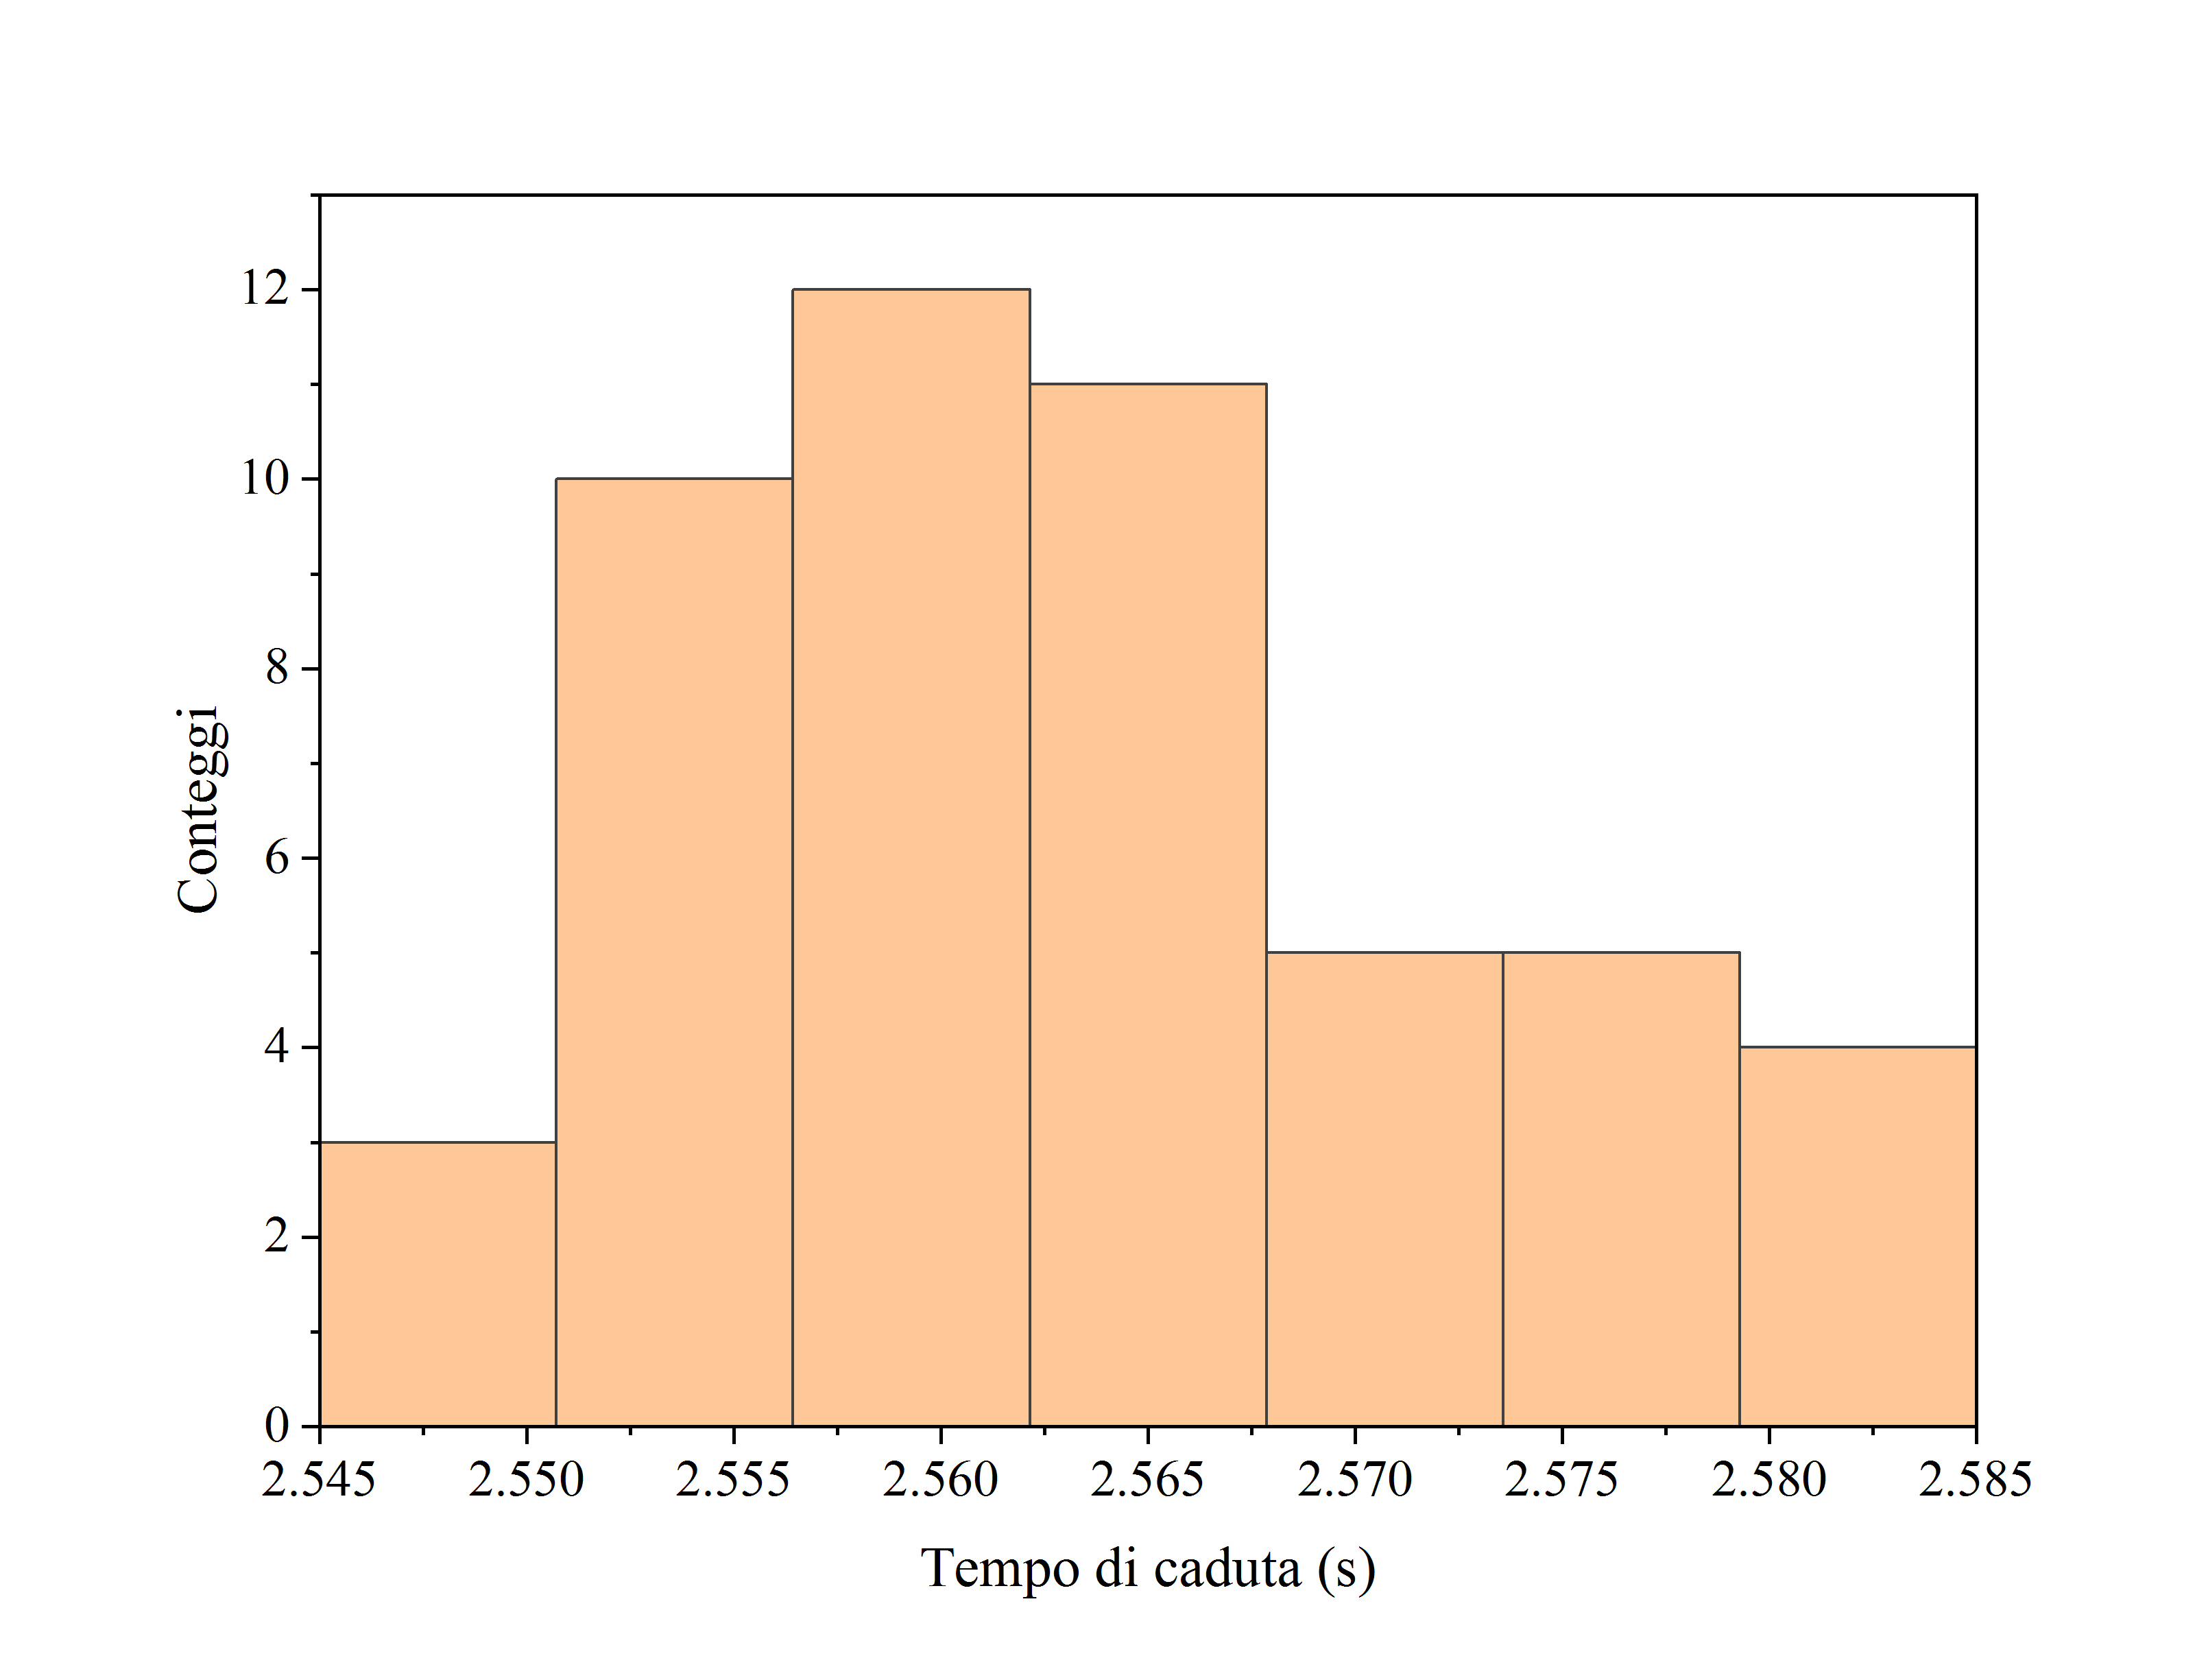
\includegraphics[trim={2.1cm 0.7cm 2.1cm 1cm},clip,width=0.47\textwidth]{img/G2.jpg}}\hfil
    \subfloat[][
        $L=(100.2\pm0.1)\;\unit{cm}$

        $\theta=(3.8\pm0.1)\unit{\degree}$
    ]{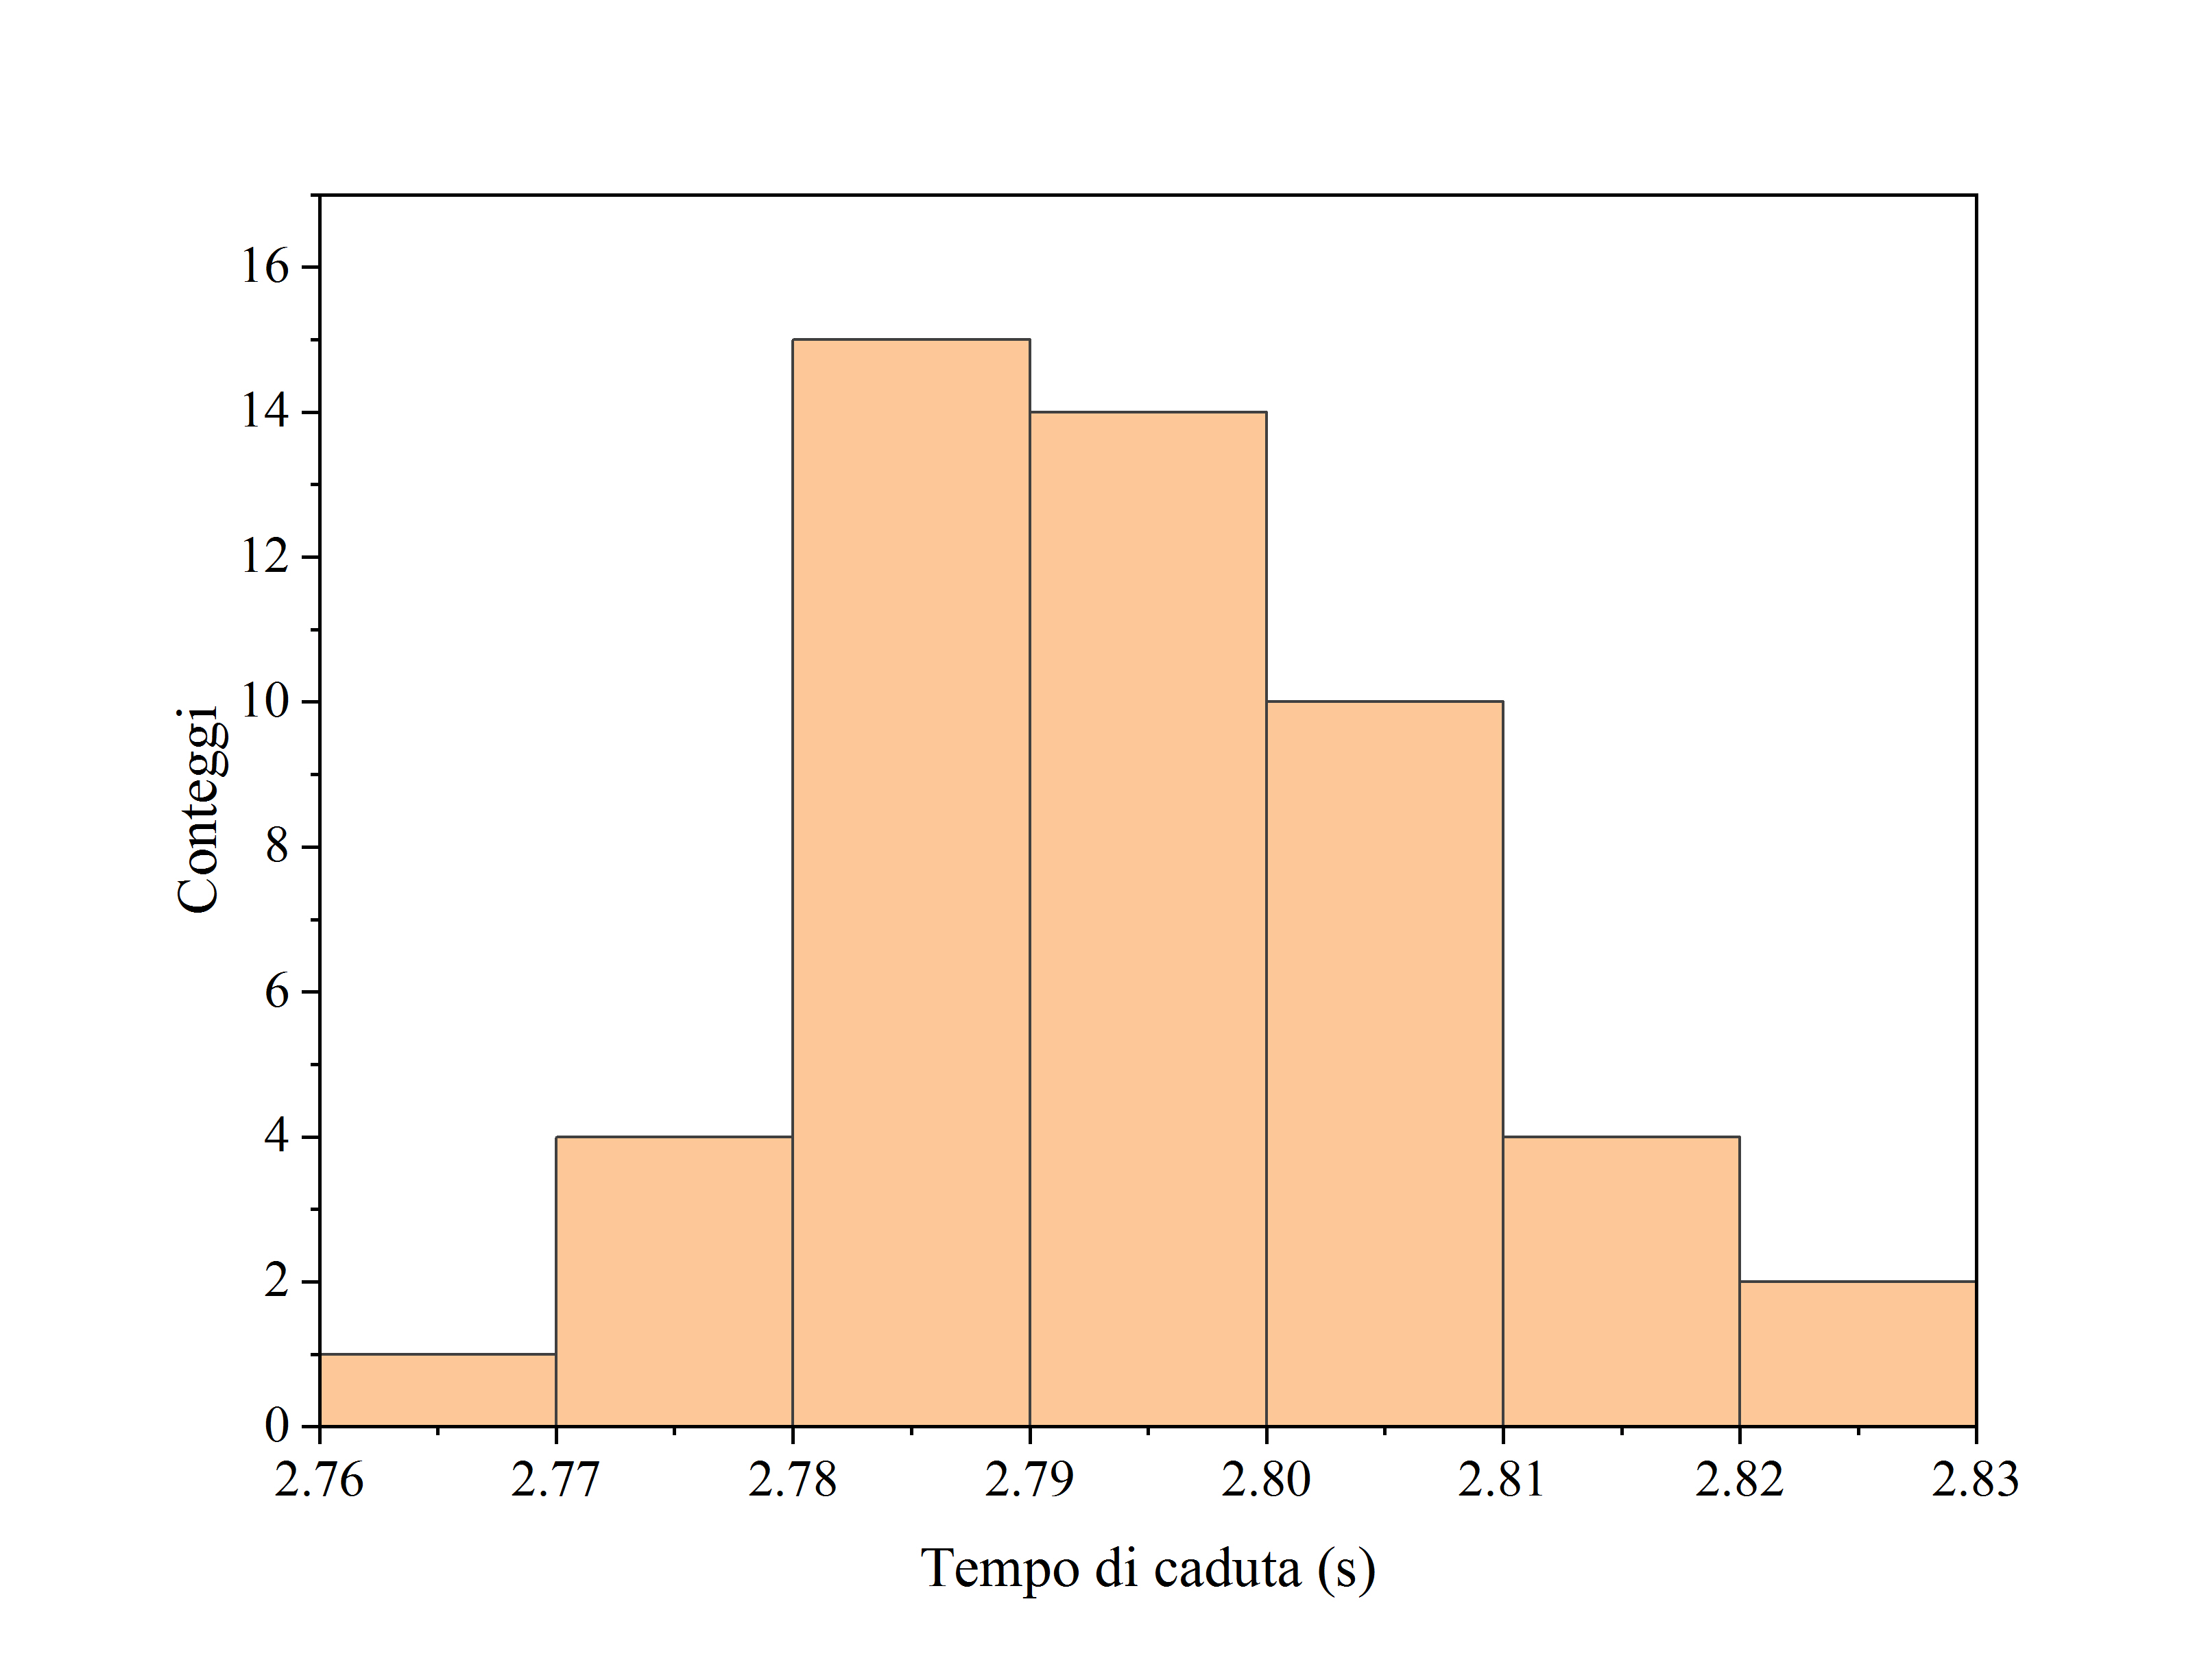
\includegraphics[trim={2.1cm 0.7cm 2.1cm 1cm},clip,width=0.47\textwidth]{img/G3.jpg}}\hfil
\end{figure}\begin{figure}[H]
    \centering
    \subfloat[][
        $L=(70.5\pm0.1)\;\unit{cm}$

        $\theta=(2.9\pm0.1)\unit{\degree}$
    ]{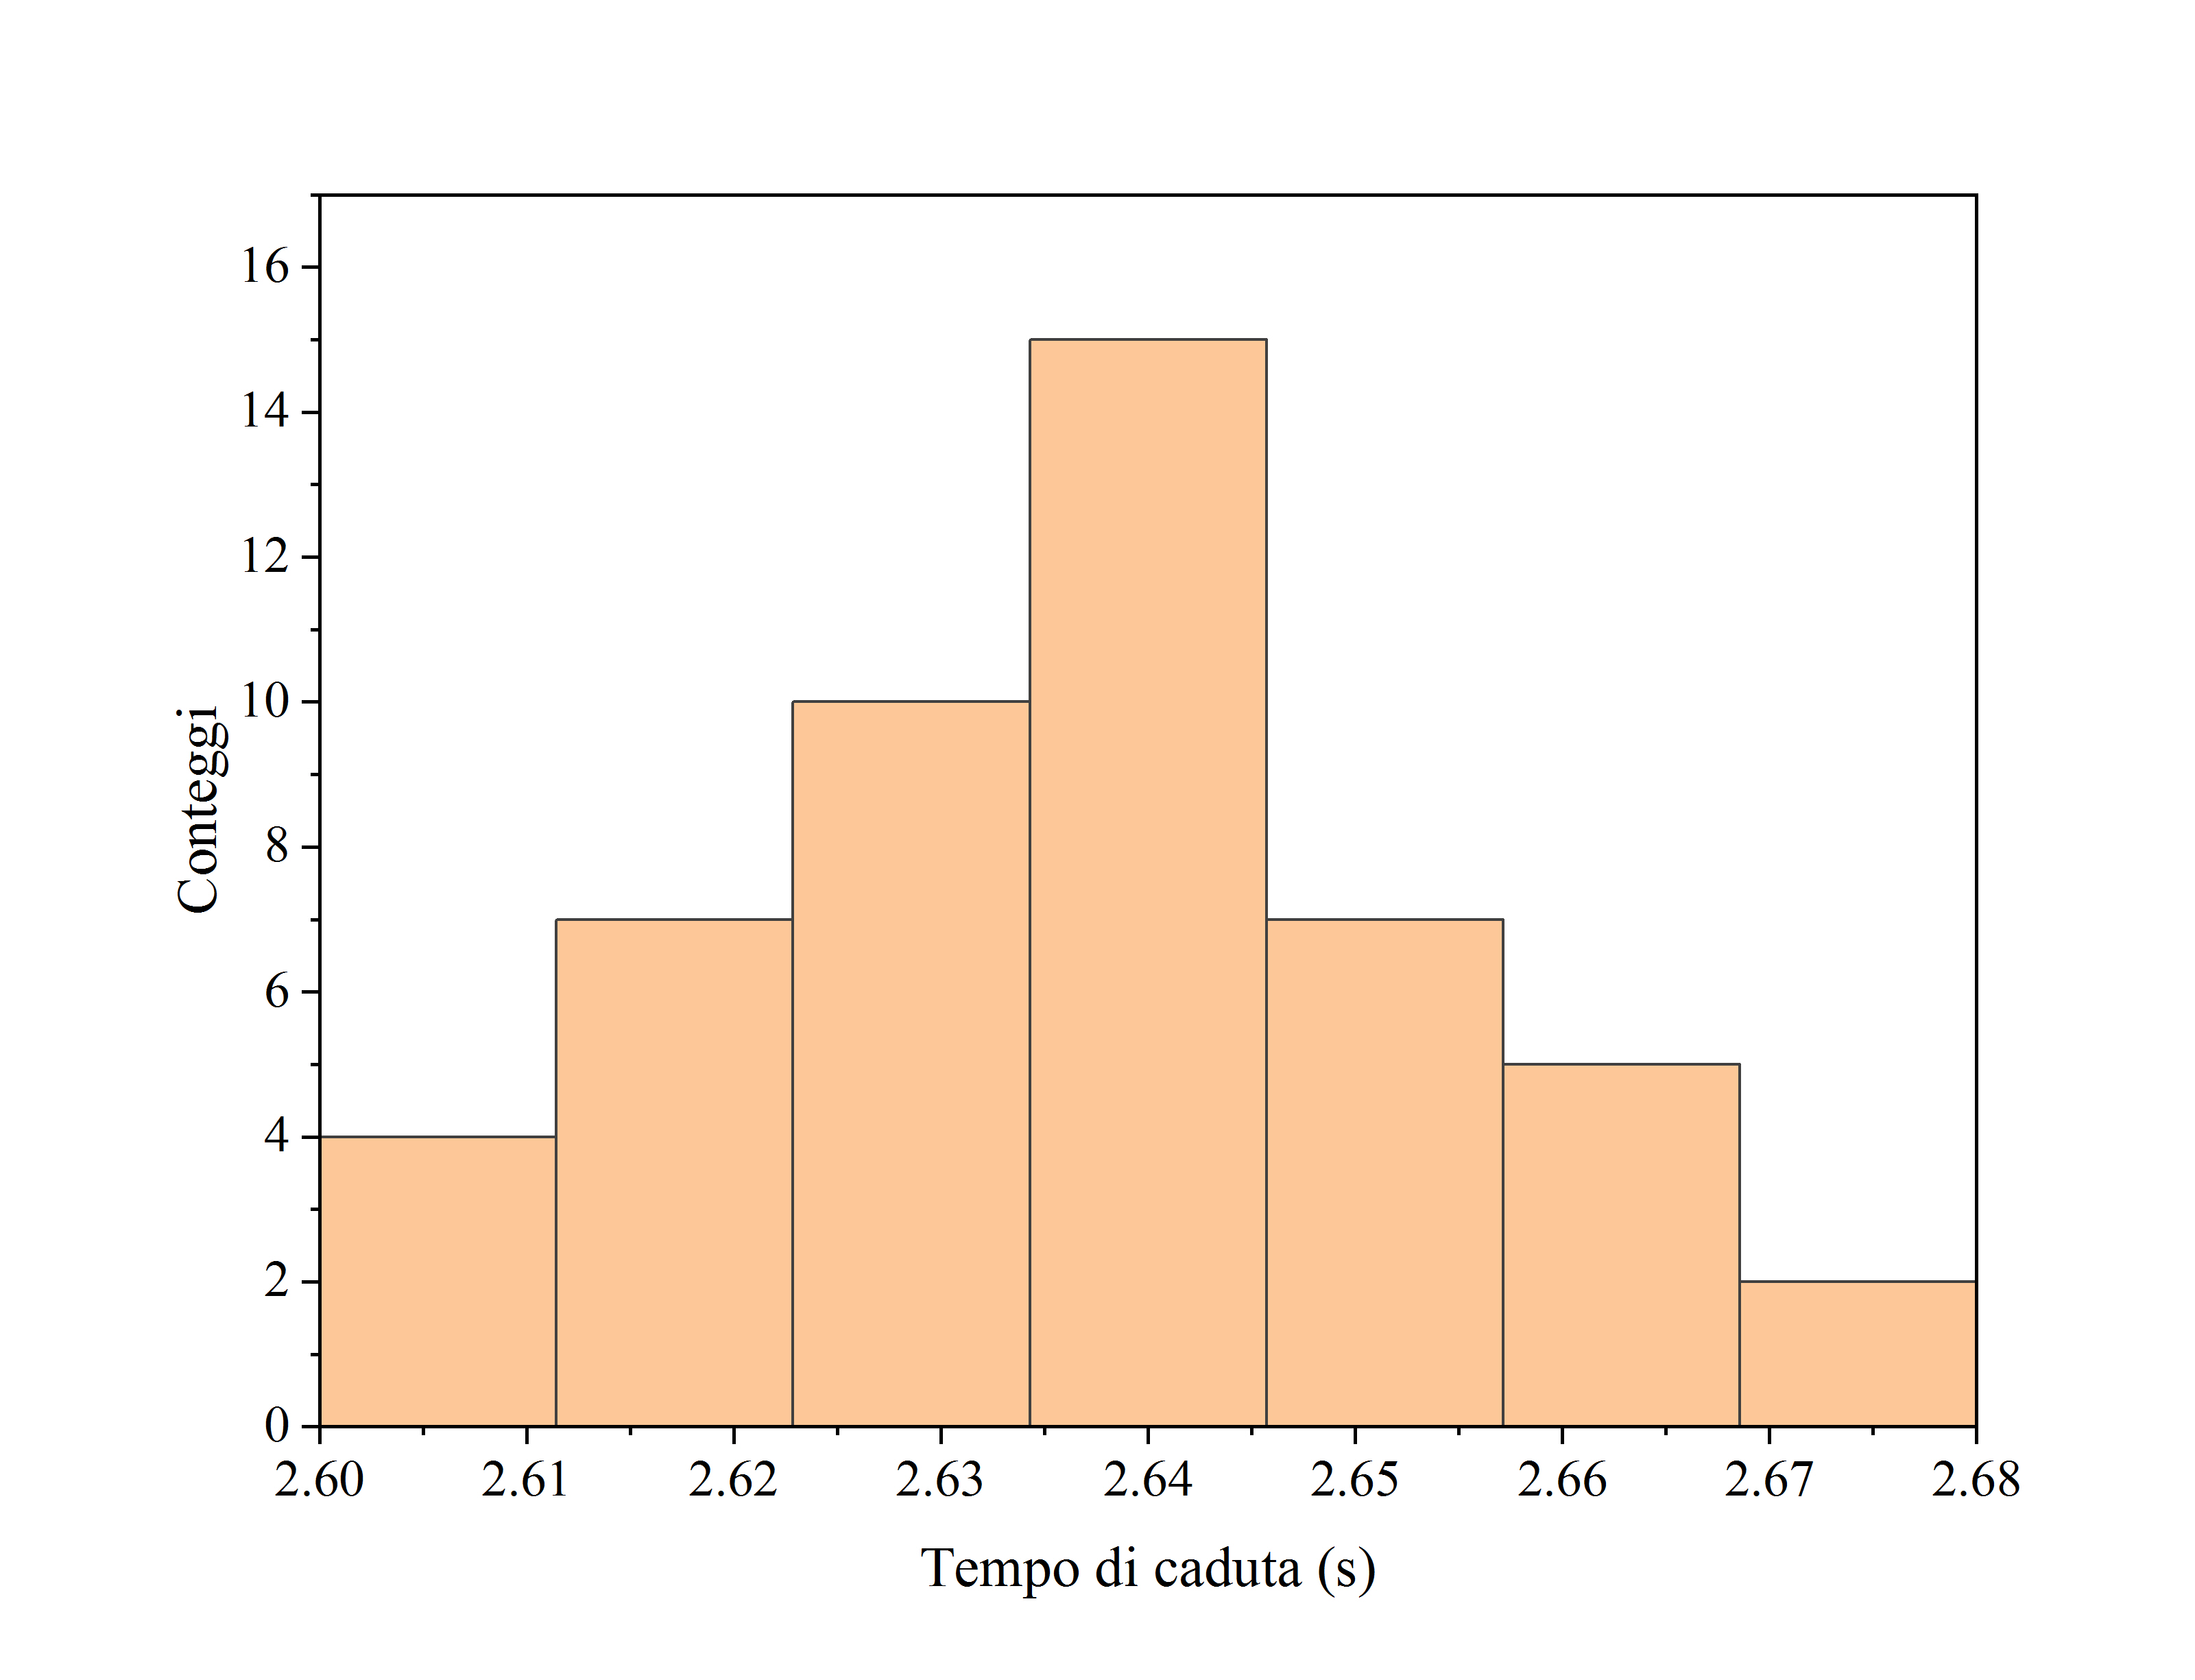
\includegraphics[trim={2.1cm 0.7cm 2.1cm 1cm},clip,width=0.47\textwidth]{img/G4.jpg}}\hfil
    \subfloat[][
        $L=(85.4\pm0.1)\;\unit{cm}$

        $\theta=(2.9\pm0.1)\unit{\degree}$
    ]{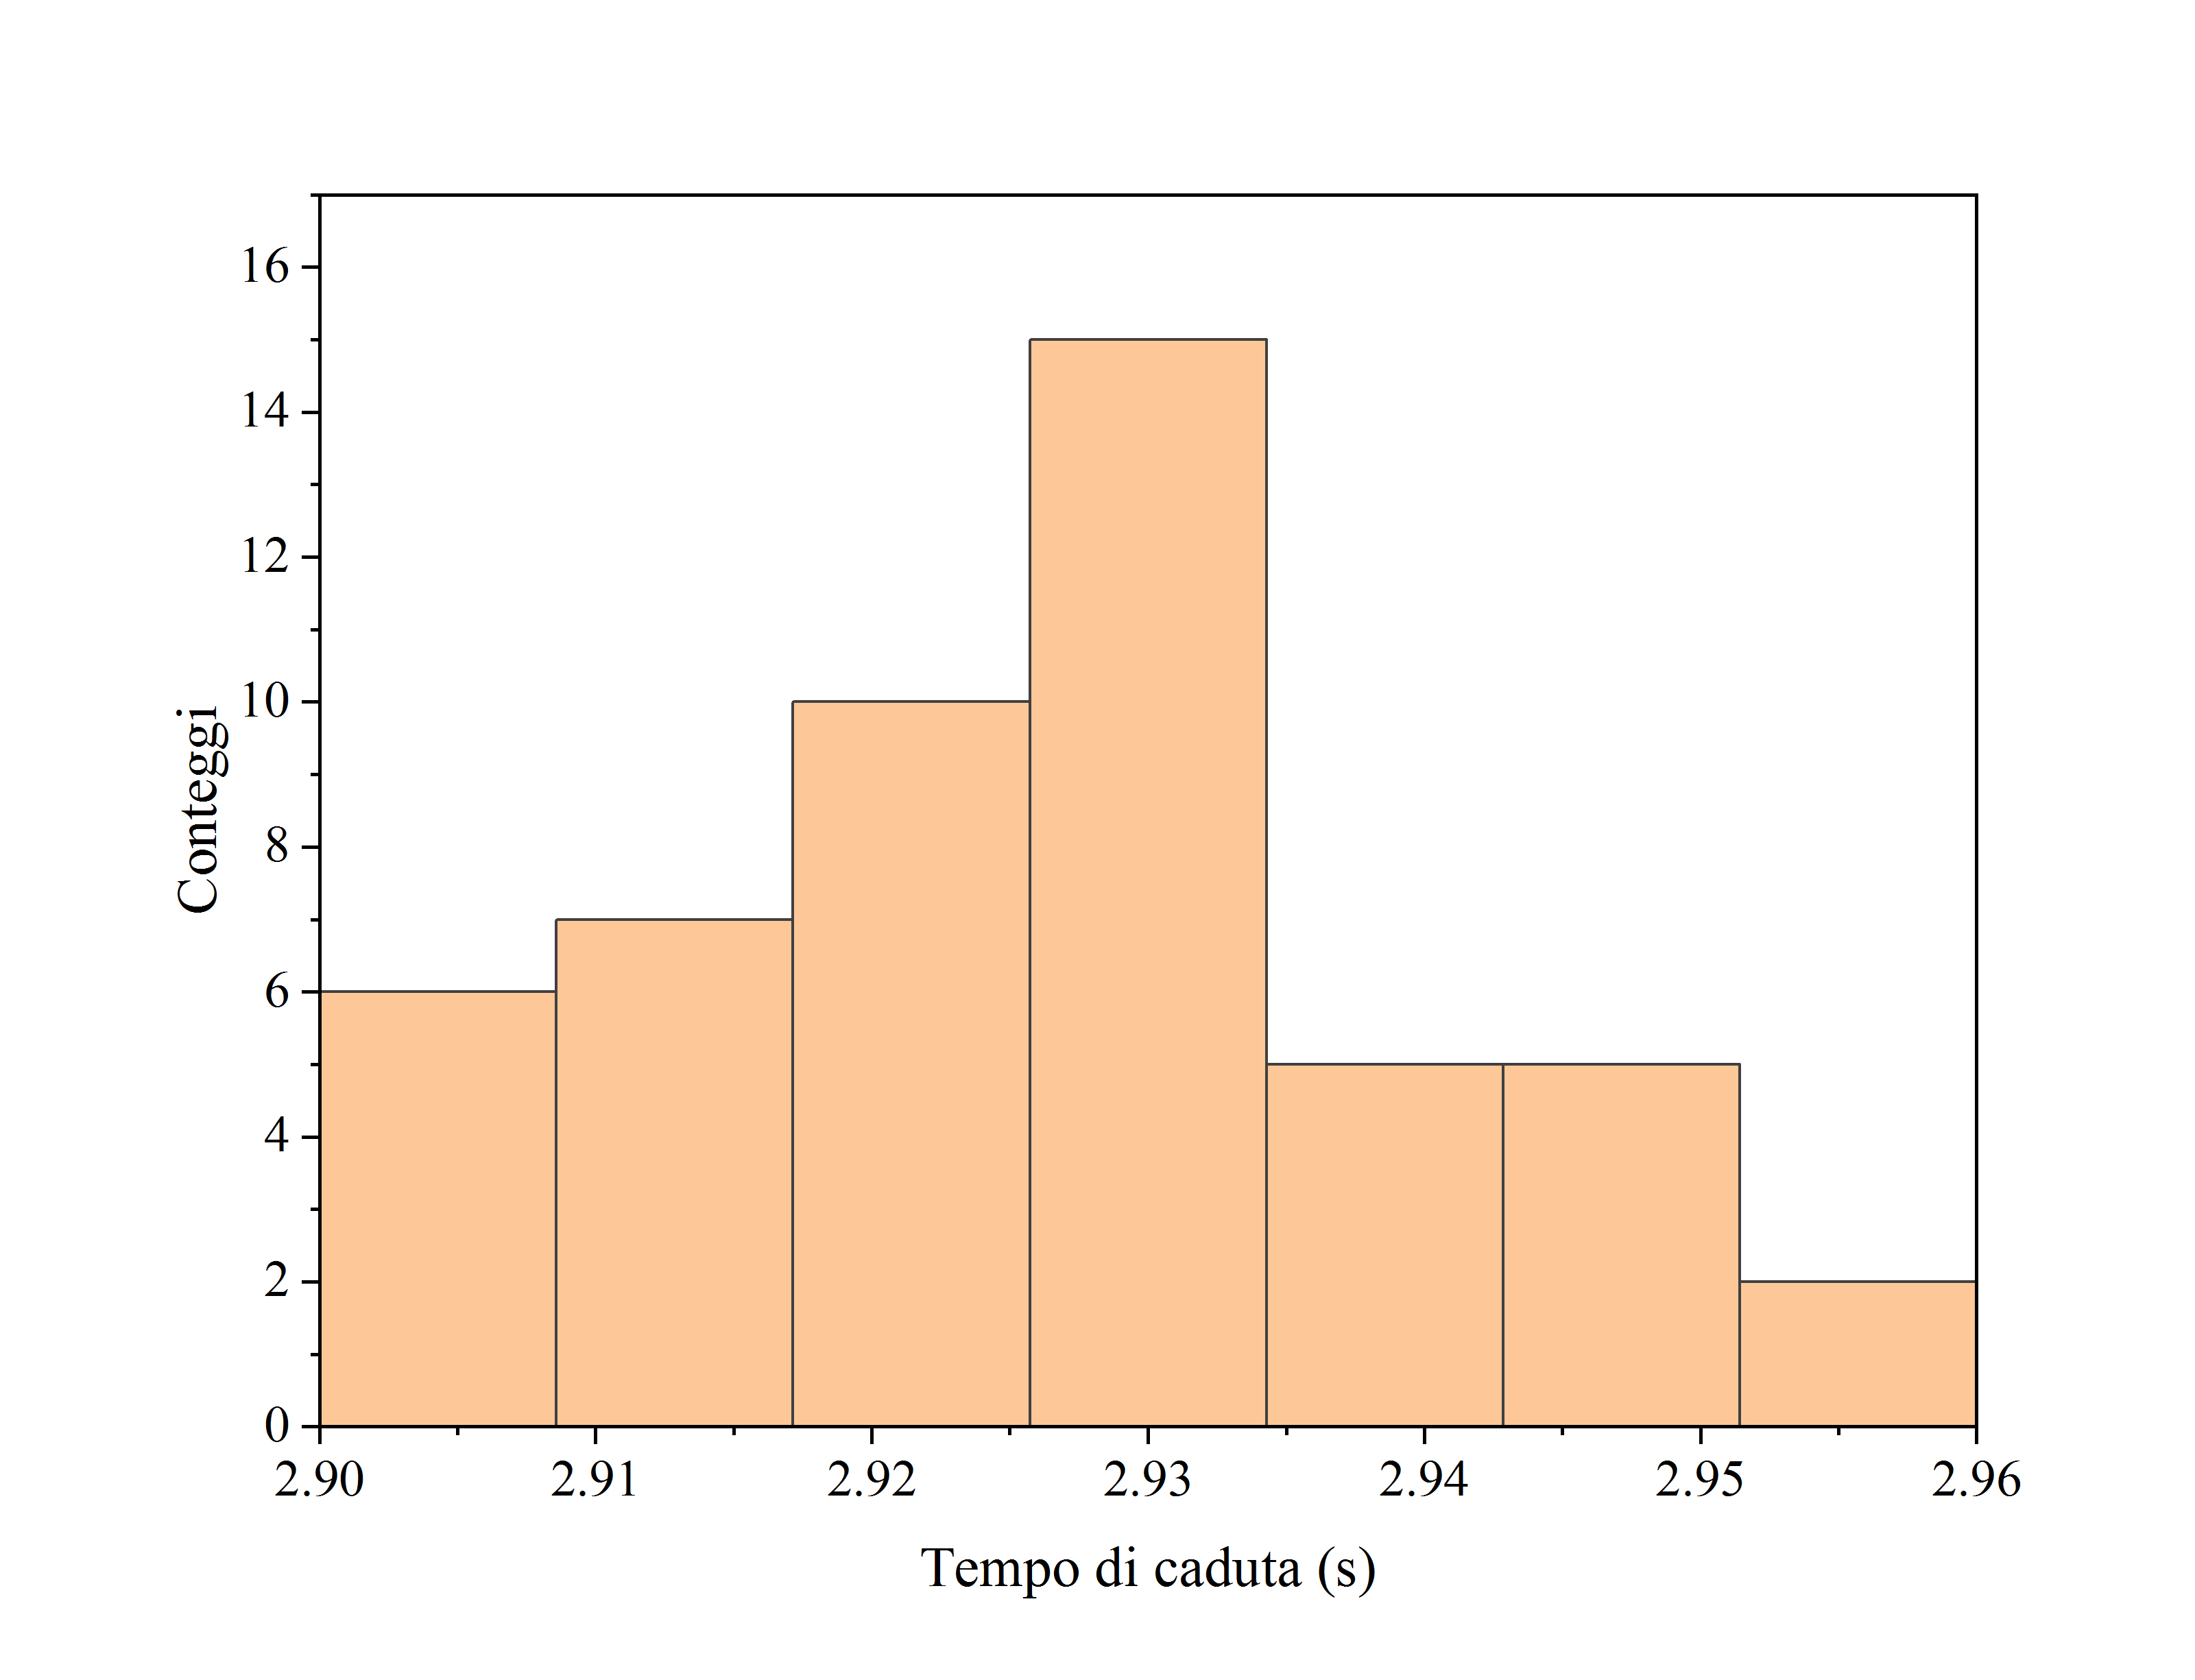
\includegraphics[trim={2.1cm 0.7cm 2.1cm 1cm},clip,width=0.47\textwidth]{img/G5.jpg}}
    \subfloat[][
        $L=(100.2\pm0.1)\;\unit{cm}$

        $\theta=(2.9\pm0.1)\unit{\degree}$
    ]{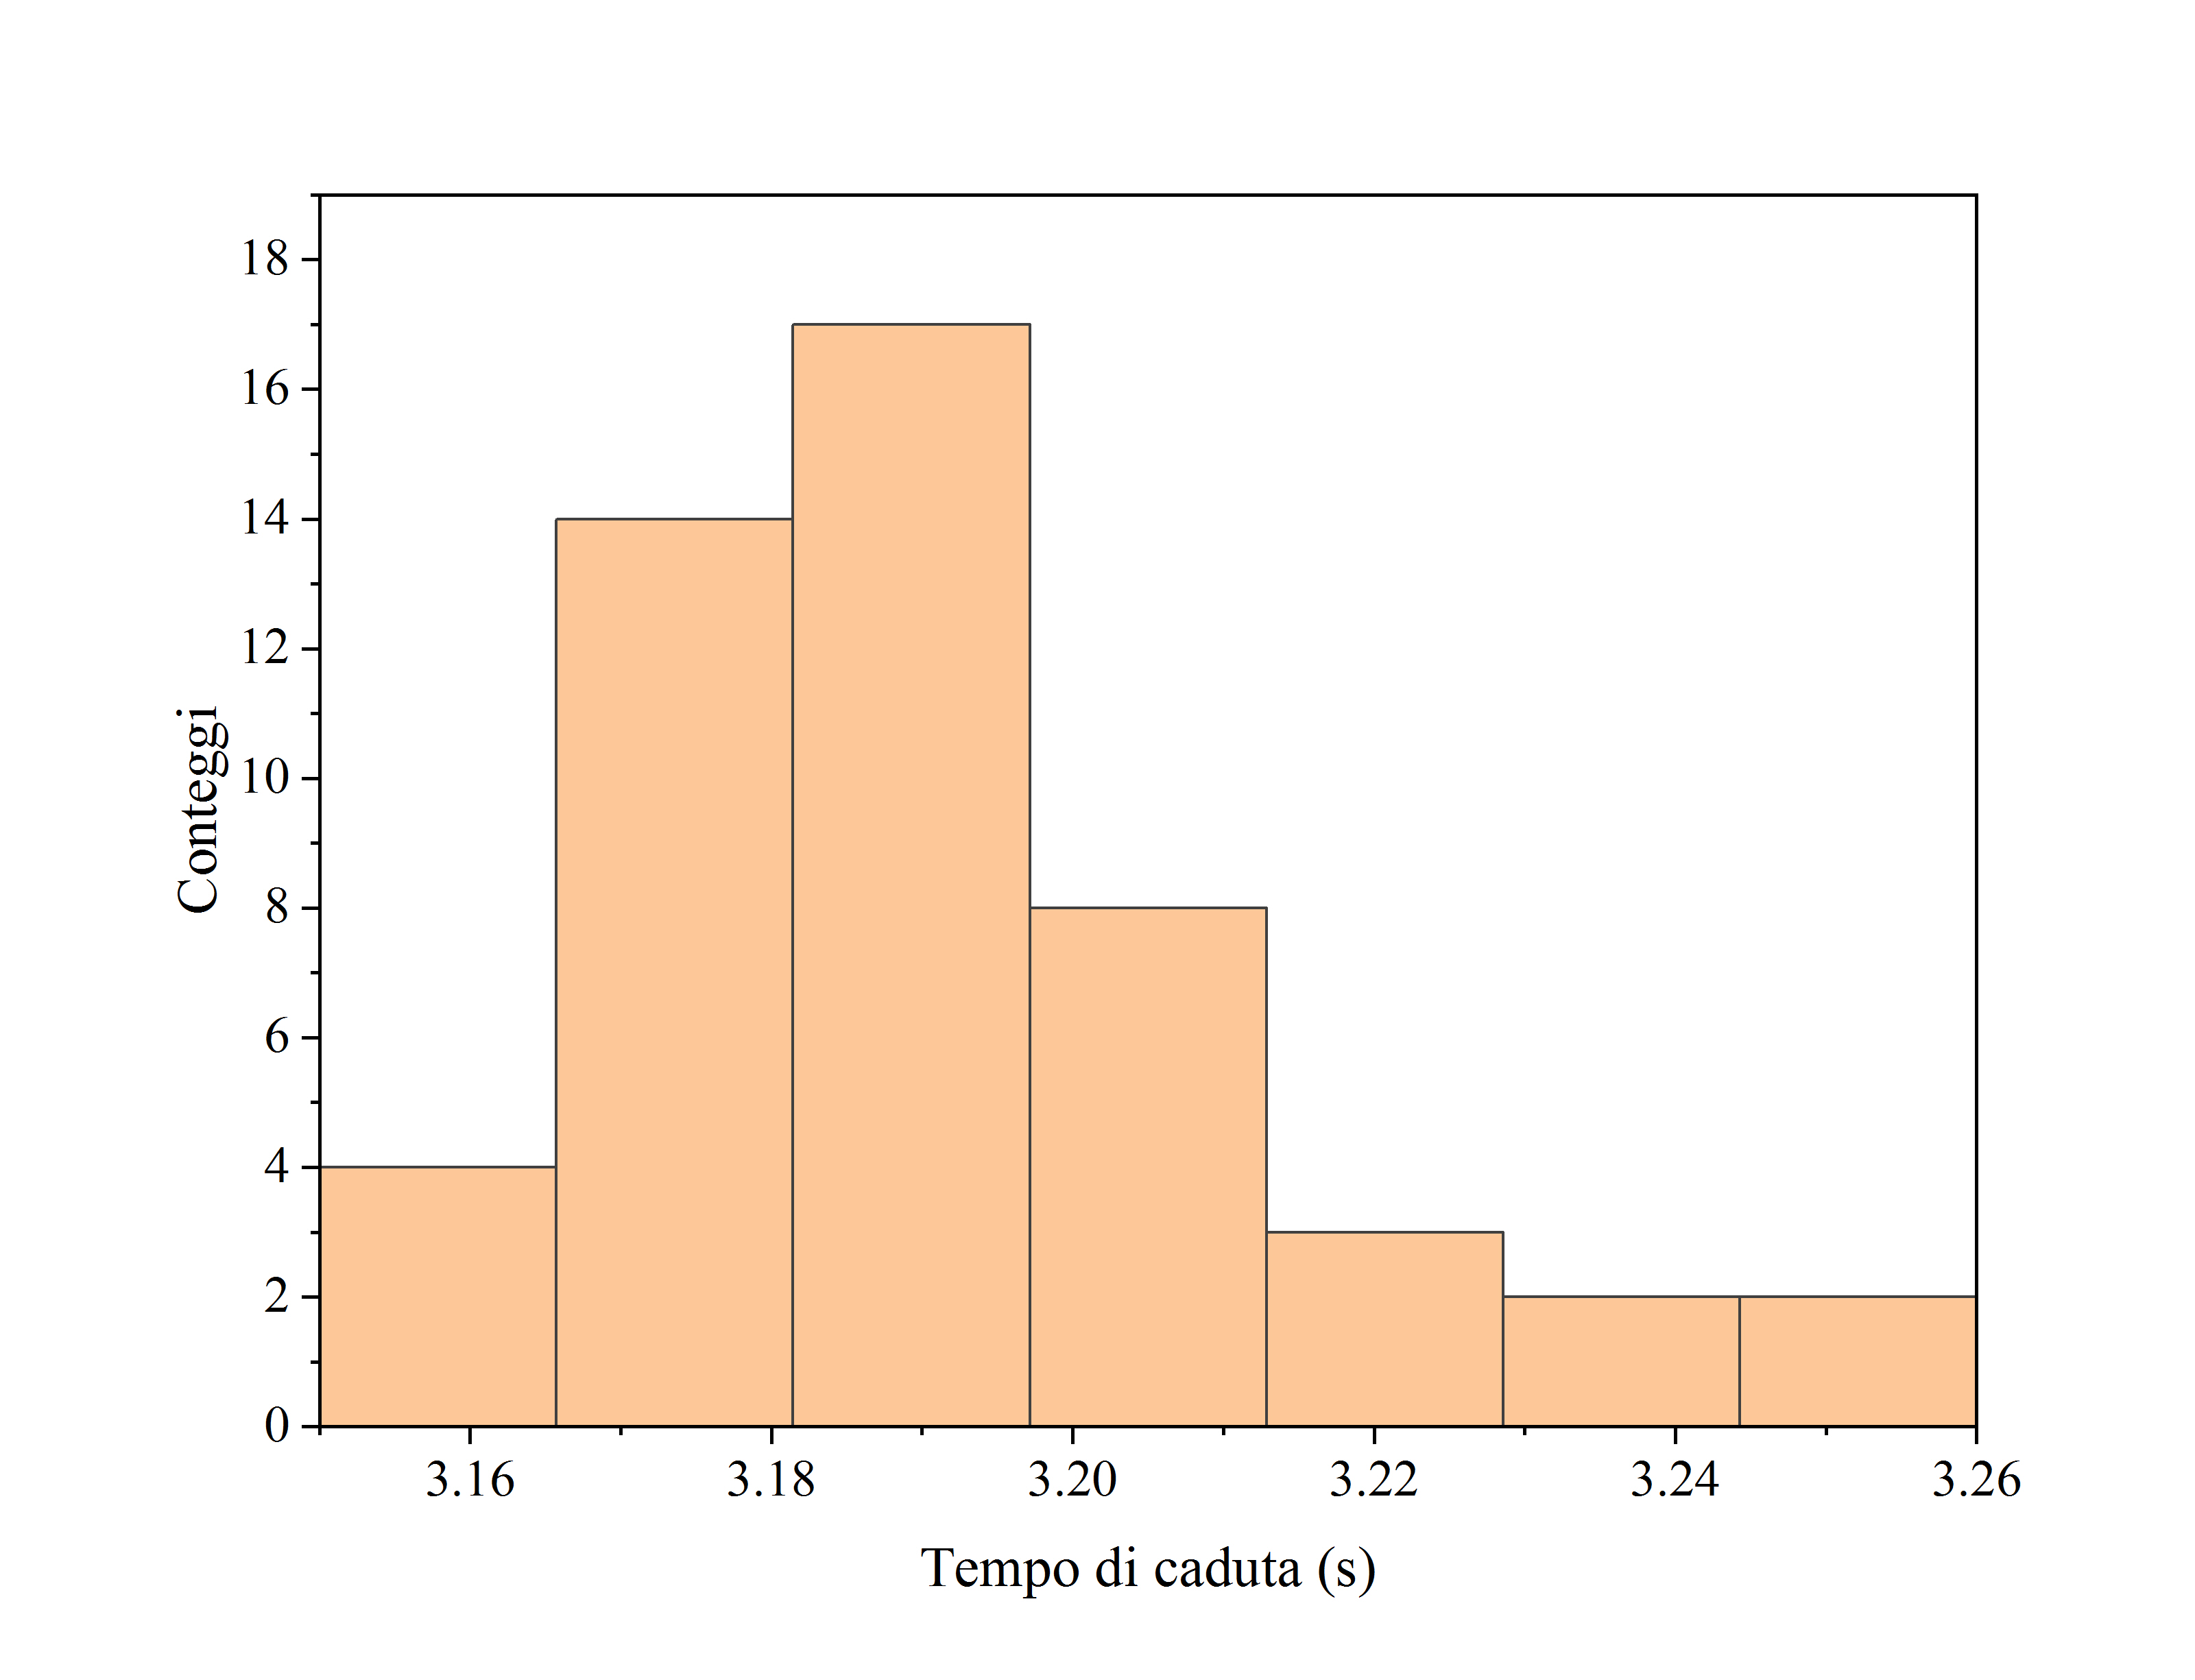
\includegraphics[trim={2.1cm 0.7cm 2.1cm 1cm},clip,width=0.47\textwidth]{img/G6.jpg}}\hfil
    \subfloat[][
        $L=(55.6\pm0.1)\;\unit{cm}$

        $\theta=(2.1\pm0.1)\unit{\degree}$
    ]{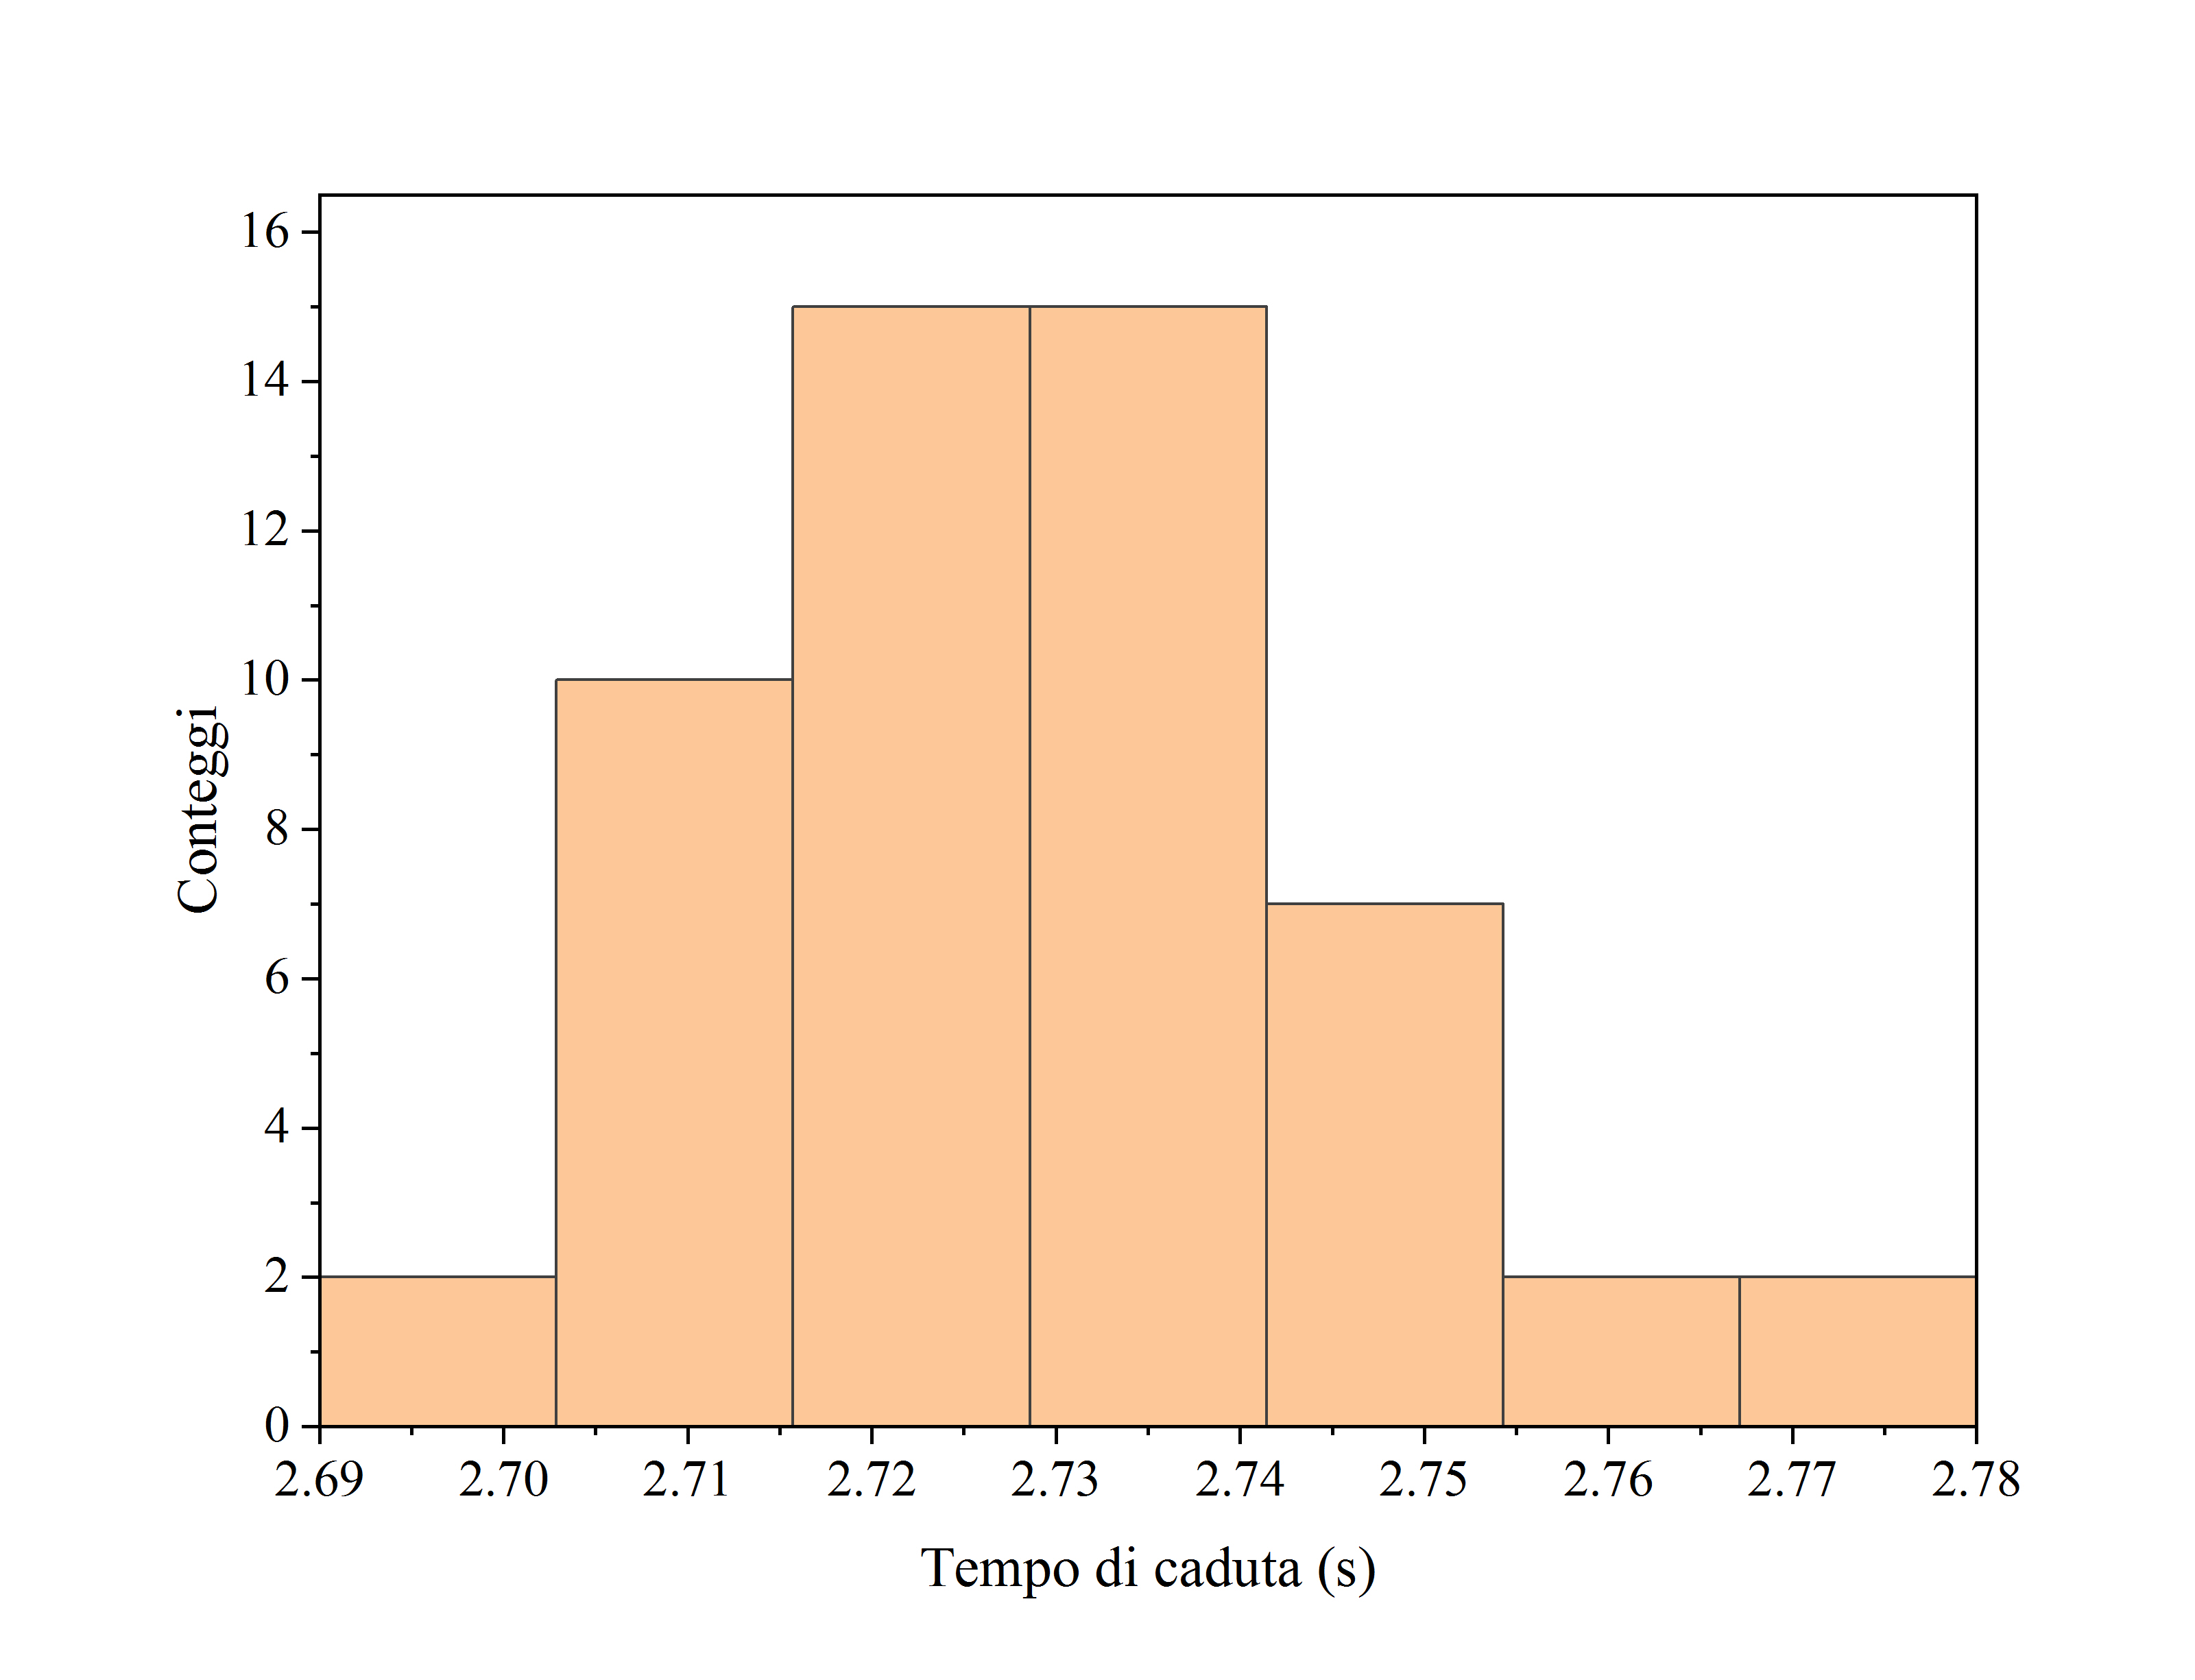
\includegraphics[trim={2.1cm 0.7cm 2.1cm 1cm},clip,width=0.47\textwidth]{img/G7.jpg}}\hfil
    \subfloat[][
        $L=(85.4\pm0.1)\;\unit{cm}$

        $\theta=(2.1\pm0.1)\unit{\degree}$
    ]{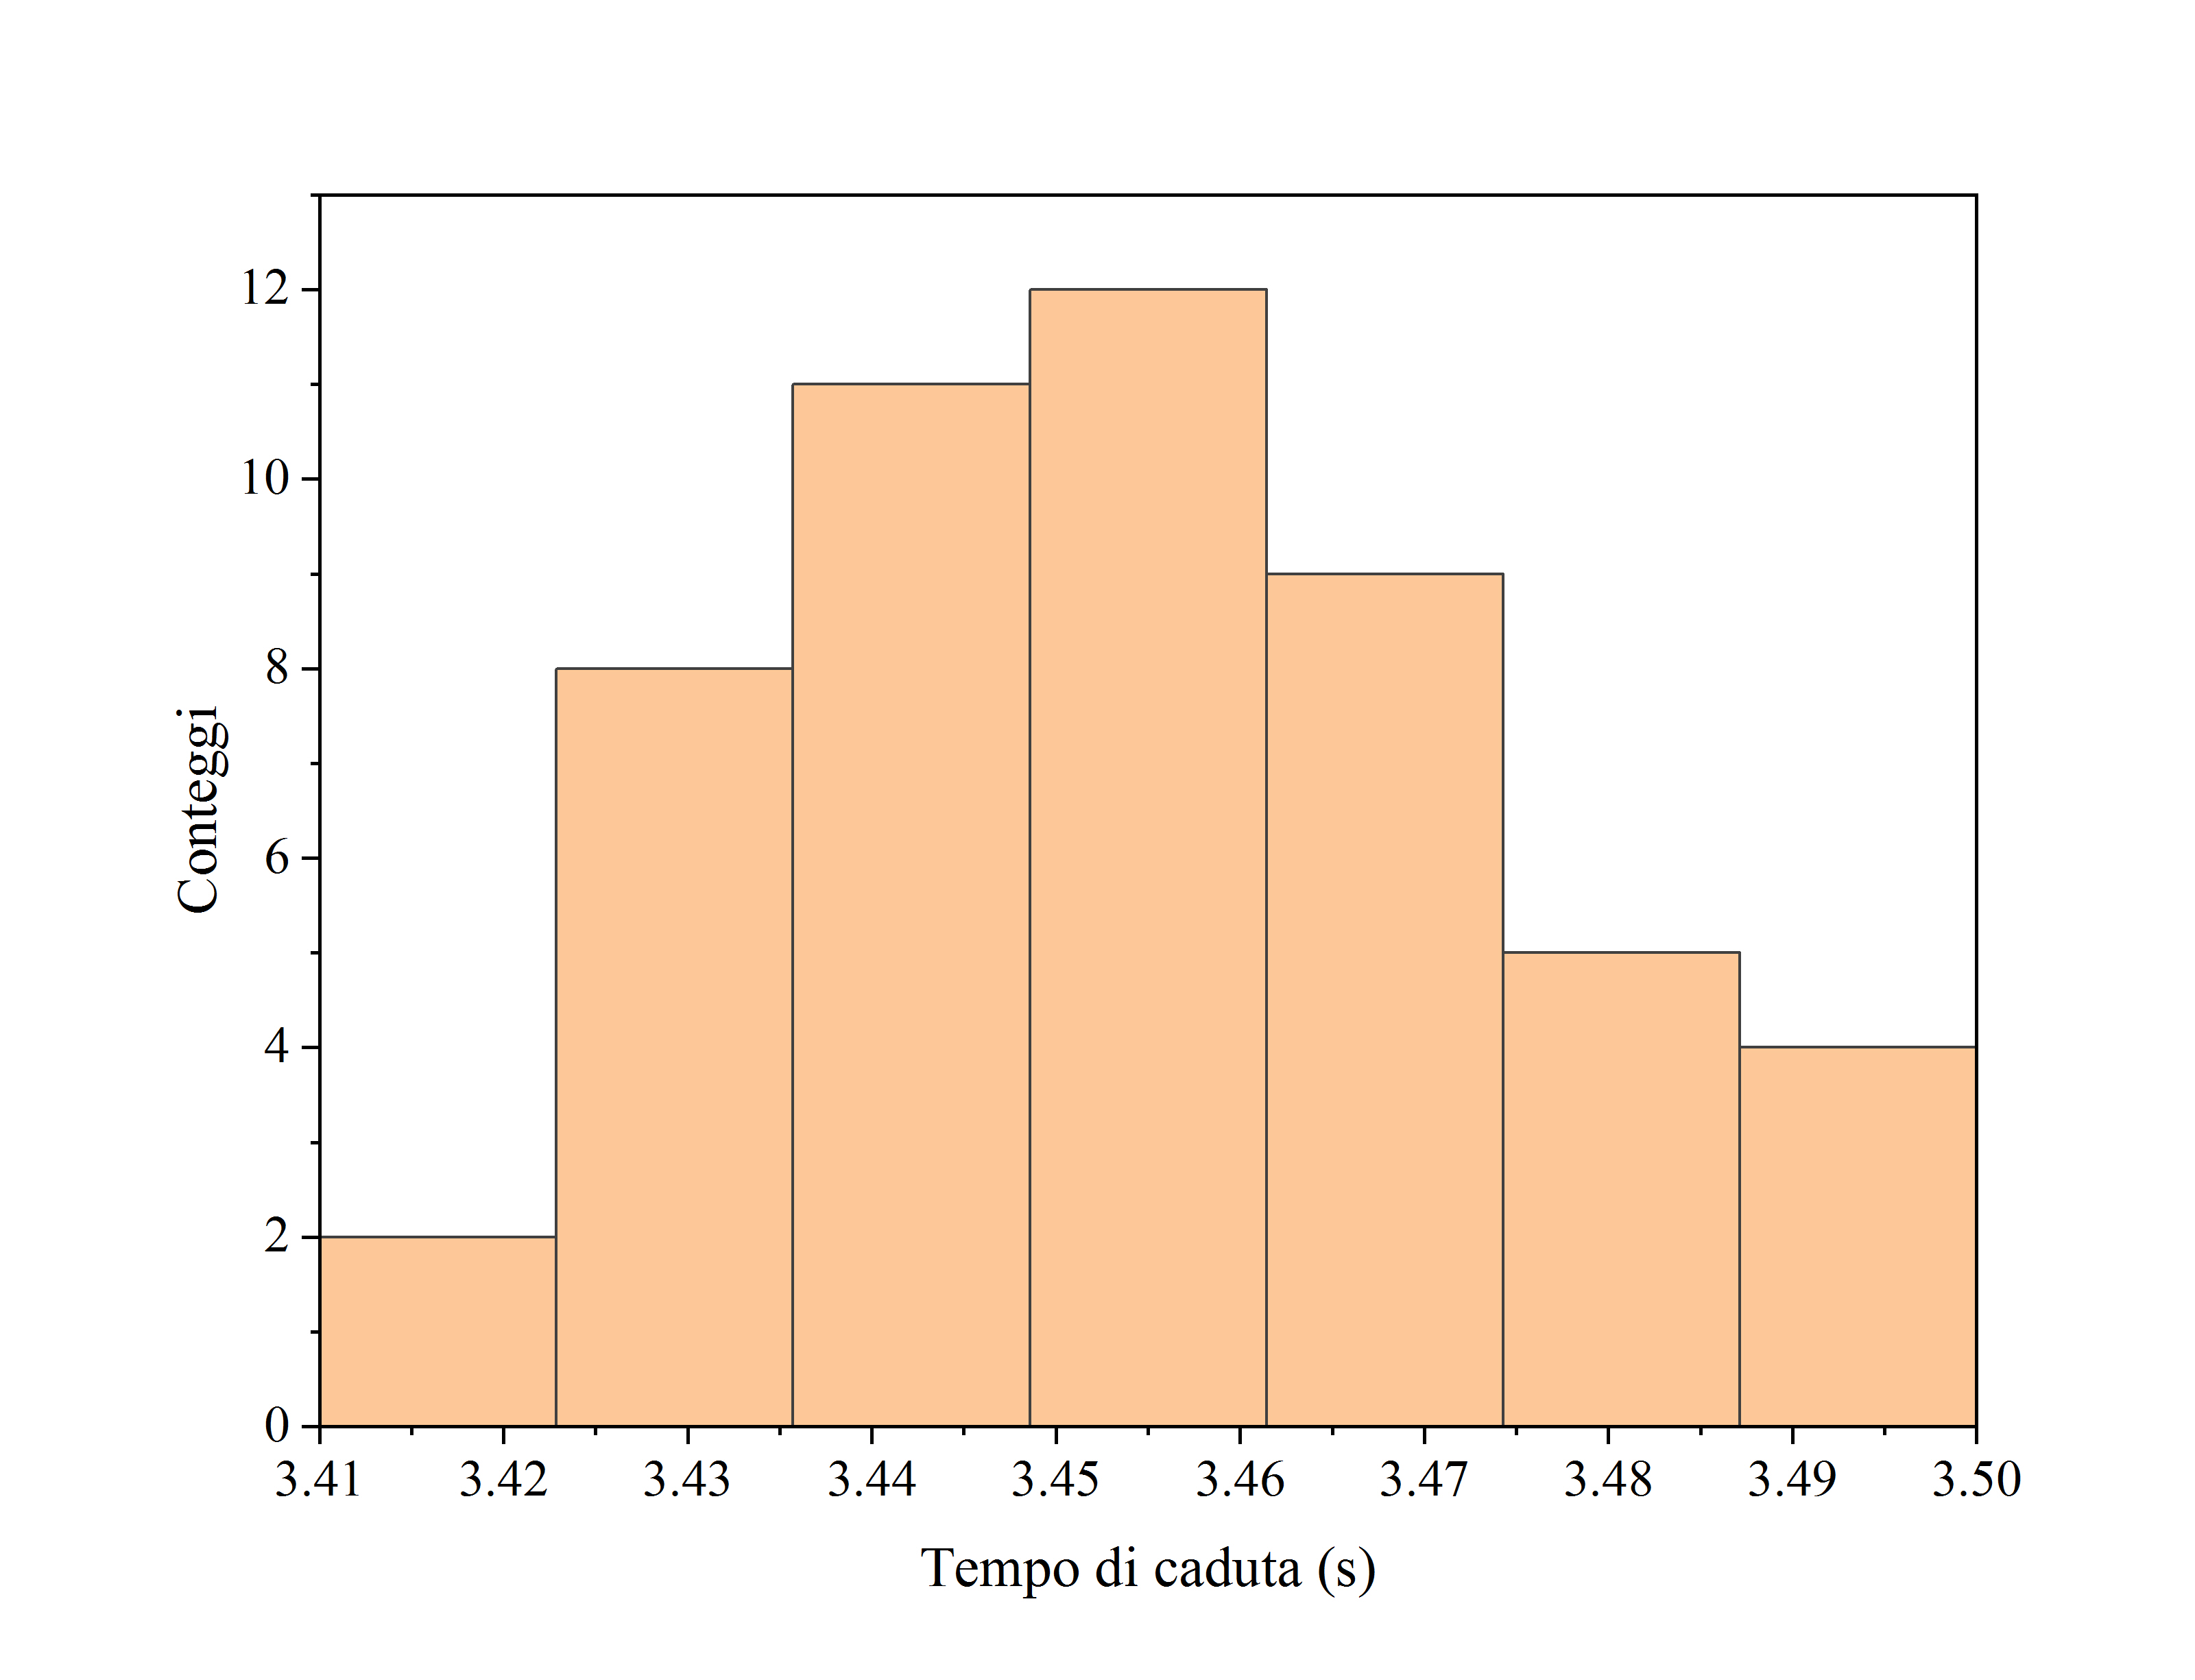
\includegraphics[trim={2.1cm 0.7cm 2.1cm 1cm},clip,width=0.47\textwidth]{img/G8.jpg}}\hfil
\end{figure}

Come è possibile osservare dai grafici qui riportati, le distribuzioni dei tempi di caduta
sono abbastanza assimilabili a distribuzioni gaussiane.
Questo ci permette di utilizzare nei calcoli successivi la media aritmetica $\bar{t}_{L,\theta}$
di ciascun set di dati, indicando come errore:
\[\sigma_{\bar{t}_{L,\theta}} = \frac{\sigma_{t_{L,\theta}}}{\sqrt{50}}\]

\subsection{Calcolo di $g$ mediante la dinamica del corpo rigido}

Fissato un sistema di riferimento cartesiano ortogonale solidale
al piano inclinato, con origine nel punto di partenza del campione,
asse $x$ parallelo alle guide e asse $y$ entrante nel piano inclinato,
possiamo scrivere la legge del moto del centro di massa e le
equazioni cardinali della dinamica del corpo rigido:
\[x_\text{CM}(t) = \frac{1}{2} a_\text{CM} t^2\]
\[\left\{\begin{aligned}
    &M g \sin\theta - F_s = M a_\text{CM} \\
    &M g \cos\theta - F_n = 0 \\
    &R M g \sin\theta = \left(I_\text{CM} + M R^2\right) \alpha
\end{aligned}\right.\]
dove $R$ è il raggio di contatto, $\vec{F}_s$ è la forza di attrito statico
tra il campione e le guide, mentre $\vec{F}_n$ è la reazione vincolare delle
guide, normale al piano.

Per poter descrivere il moto del campione come di rotolamento puro,
dobbiamo assicurarci che $F_s \le \mu_s F_n$, con $\mu_s$ il
coefficiente di attrito statico tra il corpo rigido e le guide.
Se questa condizione è verificata, possiamo utilizzare la relazione:
\[\alpha = \frac{a_\text{CM}}{R}\]

Risolvendo il sistema lineare e la disequazione di cui sopra si ottiene:
\[\left\{\begin{aligned}
    &a_\text{CM} = \frac{M R^2}{I_\text{CM} + M R^2} g\sin\theta \\
    &F_n = M g \cos\theta \\
    &F_s = \frac{I}{I + M R^2} M g \sin\theta \\
    & 0 \le \alpha \le \arctan\left(\mu_s \left(\frac{MR^2}{I_\text{CM}} + 1\right)\right) \\
\end{aligned}\right.\]

Ricordando ora che $L = x_\text{CM}(\bar{t}_{L,\theta}) + D + S$, dove $D$ è il diametro
più esterno del campione e $S$ è lo spessore del cuscinetto, possiamo ricavare:
\[
    \frac{2(L-D-S)}{\sin\theta}\left(\frac{I_\text{CM}}{M R^2} + 1\right) = g \cdot \bar{t}_{L,\theta}^2
\]

Possiamo pertanto determinare il modulo di $\vec{g}$ mediante una regressione
lineare pesata\footnote{
    La scelta di una regressione lineare \emph{pesata} è giustificata dal fatto
    che gli errori sull'ascissa, per quanto ridotti, sono diversi fra di loro.
}:
\begin{figure}[H]
    % <v>^
    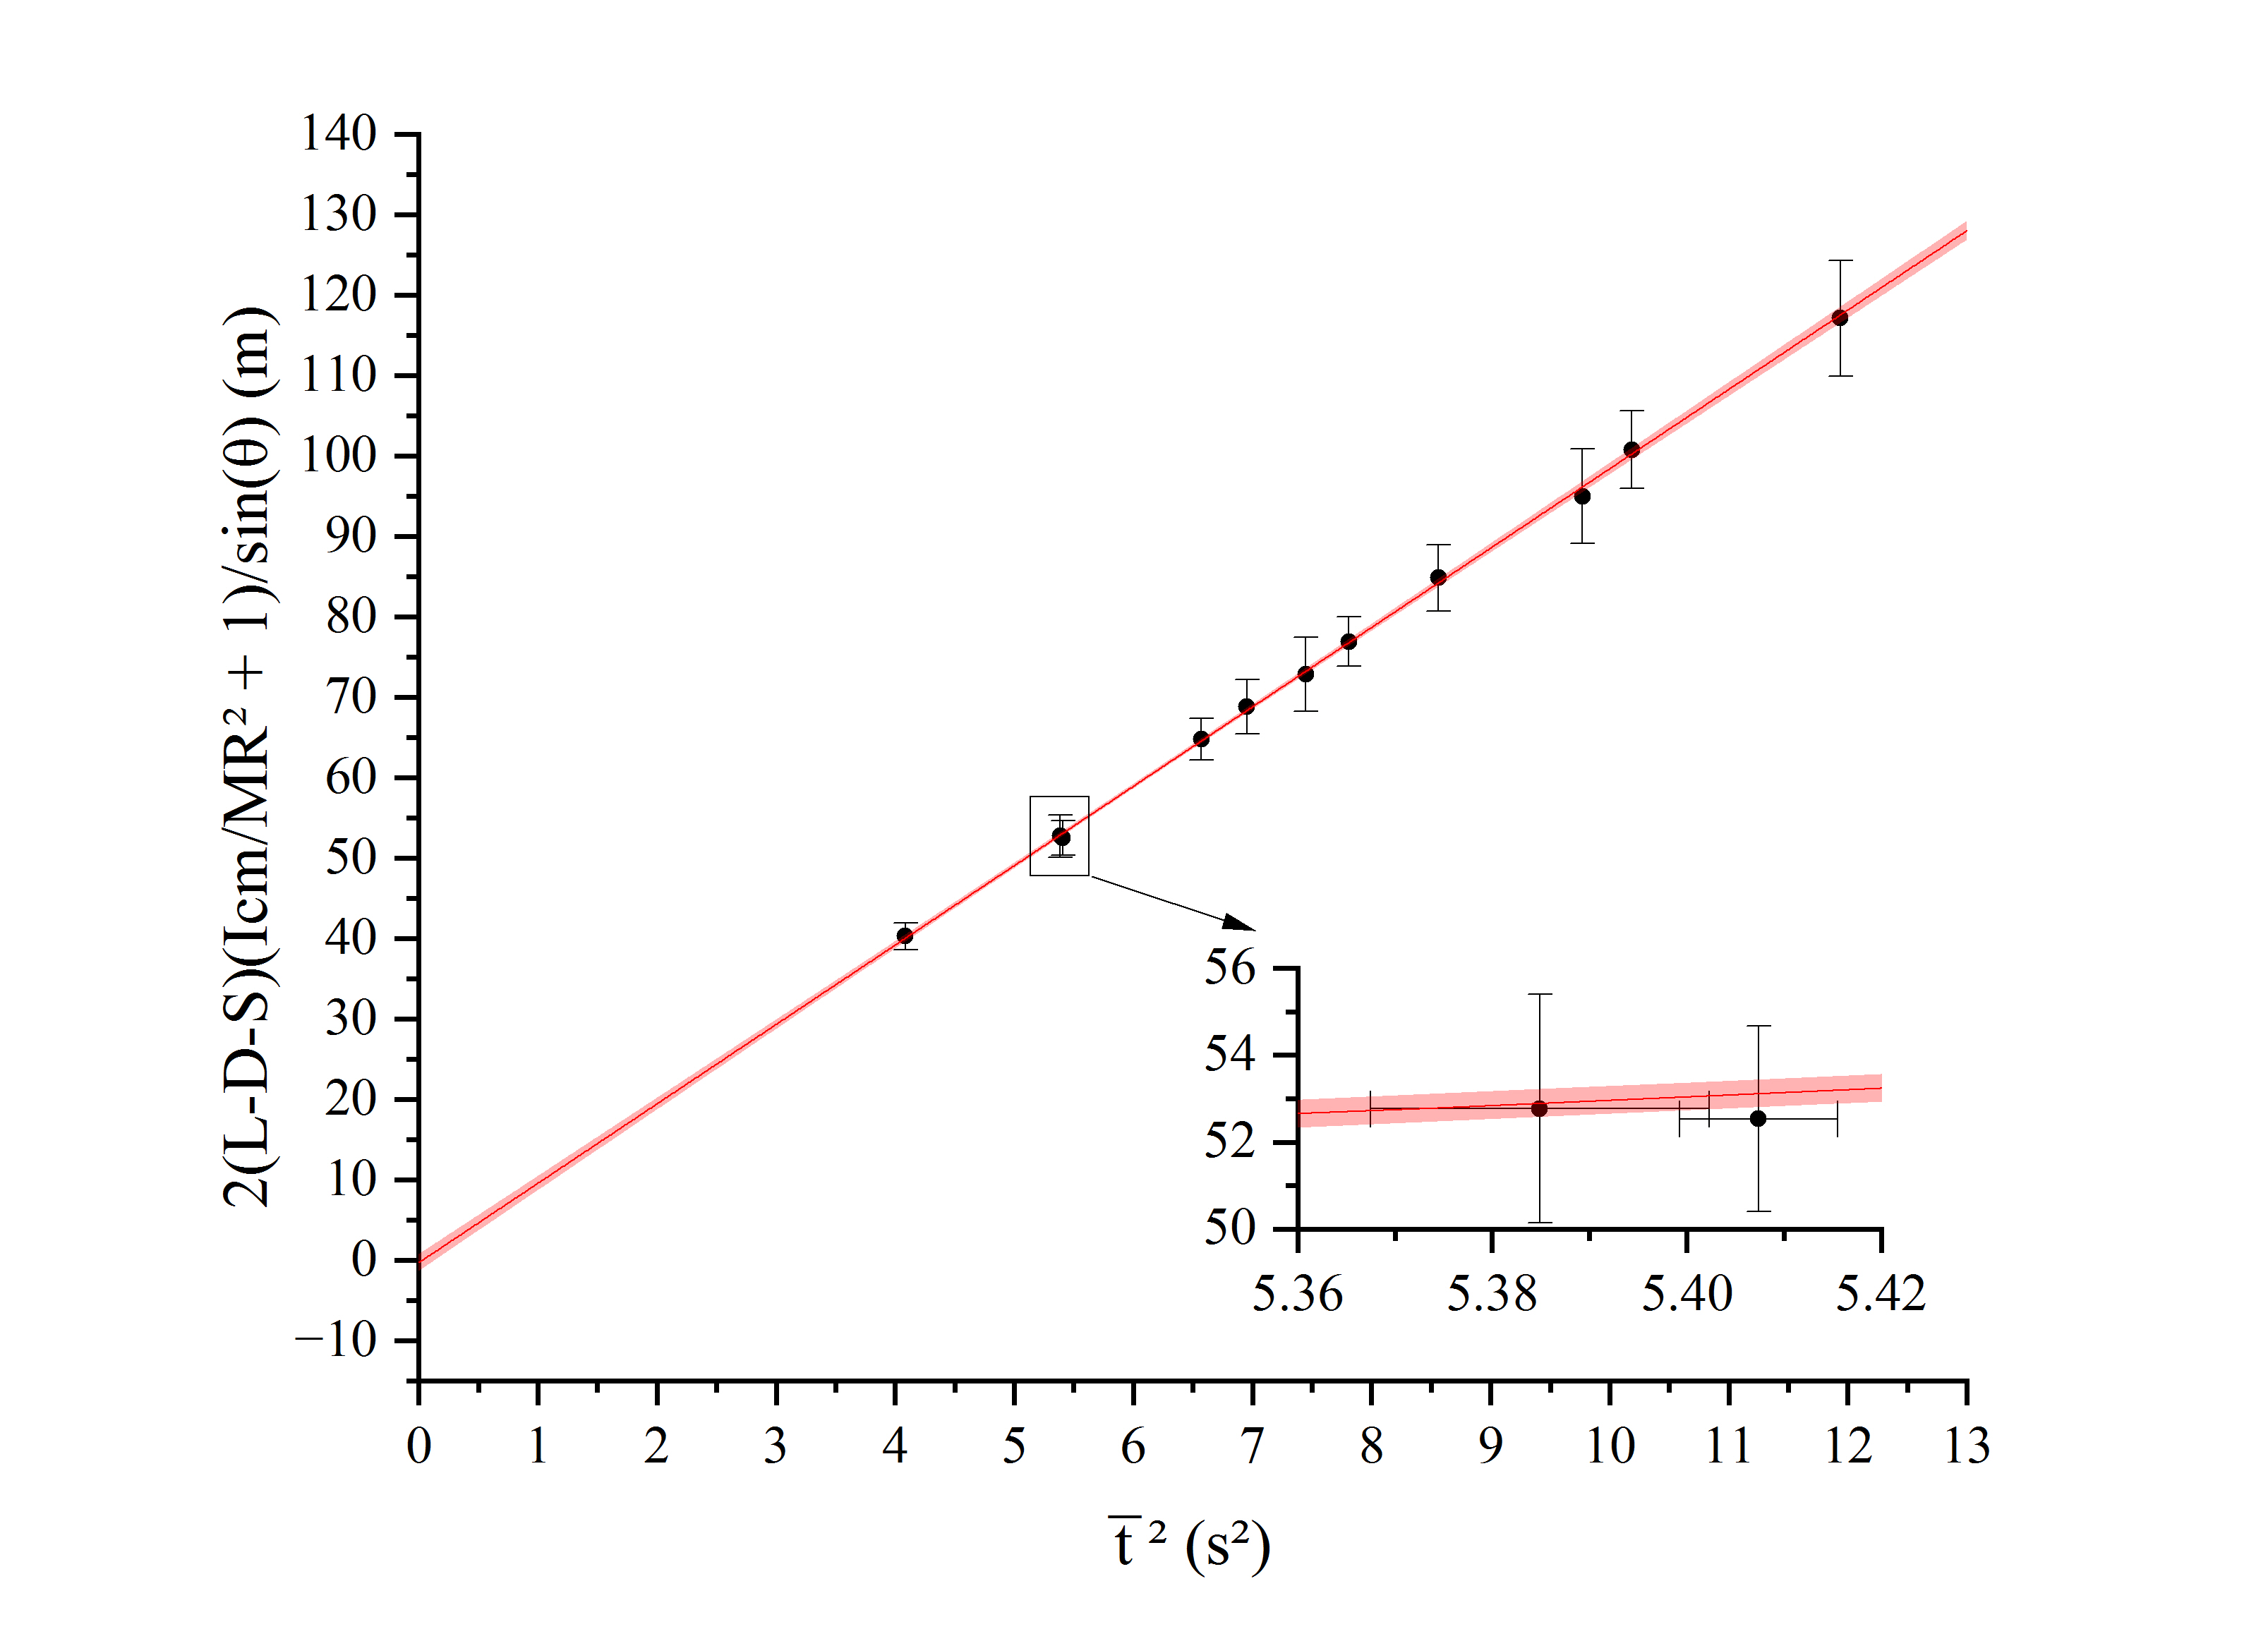
\includegraphics[trim={1cm 0.6cm 1cm 1cm},clip,width=\textwidth]{img/regressione.jpg}
    \caption*{\emph{
        In rosso la retta di regressione, in rosa la sua regione di incertezza. \\
        Le barre di errore lungo l'ascissa, date le loro dimensioni, non sono visibili.
    }}
\end{figure}

Di seguito riportiamo i risultati della regressione lineare:
\begin{itemize}
    \item Intercetta $=(0\pm3)\;\unit{m}$
    \item Coefficiente angolare ($g$) $=(9.9\pm0.5)\;\unit{m \per s^2}$
\end{itemize}

Precisiamo che gli errori su tutte le misure indirette utilizzate nella regressione lineare
sono stati calcolati mediante l'usuale metodo di propagazione degli errori: li abbiamo
infatti valutati piccoli, casuali e indipendenti.

\subsection{Conclusioni}
I risultati della regressione lineare sono chiaramente compatibili
con i valori attesi. Infatti:
\begin{itemize}
    \item Secondo il modello fisico utilizzato, l'intercetta dovrebbe essere nulla;
          in effetti, $(0\pm3)\;\unit{m}$ è compatibile con $\qty{0}{m}$.
    \item Il valore di $g$ atteso è $\qty{9.806}{m\per s^2}$; si può osservare
          facilmente che il valore misurato, $(9.9\pm0.5)\;\unit{m \per s^2}$, è
          compatibile con quello atteso.
\end{itemize}

Possiamo pertanto concludere che l'esperienza ha avuto successo: mediante l'apparato
sperimentale siamo riusciti ad ottenere una misura di $g$ compatibile con quella attesa.

Precisiamo che non è certo da escludere la presenza di errori sistematici: si può infatti
osservare come le distribuzioni dei tempi di caduta tendano ad essere un po' asimmetriche,
in particolare “più spostate” verso tempi più bassi.

Tuttavia, alla luce dei risultati della regressione lineare, il gruppo di lavoro ritiene
che, comunque, questi errori non siano significativi.

\end{document}
